%----------------------------------------------------------------------------------------
%   PACKAGES AND DOCUMENT CONFIGURATIONS
%----------------------------------------------------------------------------------------

\documentclass[captions=tableheading,a4paper,11pt,numbers=noenddot,titlepage,twoside,openright,DIV=14,BCOR=8mm,parskip=half]{scrbook}
\PassOptionsToPackage{obeyspaces}{url}
\usepackage[backend=biber,
            autocite=plain,
            sorting=none,
            url=false
            ]{biblatex}
\usepackage[headsepline]{scrlayer-scrpage}
\usepackage[T1]{fontenc}
\usepackage[shortlabels]{enumitem}
\usepackage{siunitx}
\usepackage{array}
\usepackage{ccicons}
\usepackage{booktabs}
\usepackage{xspace}
\usepackage{xcolor}
\usepackage{minted}
\usepackage{a4wide}
\usepackage{listings}
\usepackage{graphicx}
\usepackage{seqsplit}
\usepackage{multirow}
\usepackage[unicode=true]{hyperref}
\usepackage{microtype}
\usepackage{pgffor}
\usepackage{lmodern}
\usepackage{amssymb,amsmath}
\usepackage{ifxetex,ifluatex}
\usepackage{fixltx2e}
\usepackage[utf8]{inputenc}
\usepackage{eurosym}
\usepackage{fancyvrb}
\urlstyle{same}
\usepackage{longtable,booktabs}
\usepackage[normalem]{ulem}

\setlength{\emergencystretch}{3em}
\providecommand{\tightlist}{%
  \setlength{\itemsep}{0pt}\setlength{\parskip}{0pt}}

\ifx\paragraph\undefined\else
\let\oldparagraph\paragraph
\renewcommand{\paragraph}[1]{\oldparagraph{#1}\mbox{}}
\fi
\ifx\subparagraph\undefined\else
\let\oldsubparagraph\subparagraph
\renewcommand{\subparagraph}[1]{\oldsubparagraph{#1}\mbox{}}
\fi

\providecommand{\subtitle}[1]{}

\pagestyle{scrheadings}
\lehead{\leftmark}
\rohead{\rightmark}
\lefoot{\pagemark}
\rofoot{\pagemark}

% Set paths
\makeatletter
\def\input@path{{usermanual/}}
\makeatother

% Load configuration
% Set bibliography
\addbibresource{usermanual/references.bib}

% Set allpix version
\newcommand{\version}{\lstinline|@ALLPIX_VERSION@|}
\newcommand{\project}{@CMAKE_PROJECT_NAME@}


\renewcommand*{\titlepagestyle}{empty}
%----------------------------------------------------------------------------------------
%   DOCUMENT INFORMATION
%----------------------------------------------------------------------------------------
\titlehead{\centering
\includegraphics[width=7cm]{logo.png}}
\title{\apsqbold User Manual} % Title

\author{Koen Wolters (\href{mailto:koen.wolters@cern.ch}{koen.wolters@cern.ch})\\
  Simon Spannagel (\href{mailto:simon.spannagel@cern.ch}{simon.spannagel@cern.ch})\\
  Daniel Hynds (\href{mailto:daniel.hynds@cern.ch}{daniel.hynds@cern.ch})
} % Author names

\date{\today\\ \vspace{10pt} Version \version} % Date for the report

\graphicspath{{usermanual/figures/}}

\begin{document}
\begin{titlepage}
\maketitle % Insert the title, author and date

\addlicense
\end{titlepage}

\cleardoublepage
% Table Of Contents
\tableofcontents

\cleardoublepage

% intro
\section{Introduction}
\label{sec:introduction}
\apsq is a generic simulation framework for silicon tracker and vertex detectors written in modern C++.
It is the successor of a previously developed simulation framework called AllPix~\cite{ap1wiki,ap1git}.
The goal of the \apsq framework is to provide and easy-to-use package for simulating the performance of Silicon detectors, starting with the passage of ionizing radiation through the sensor and finishing with the the digitization of hits in the readout chip.

The framework builds upon other packages to perform tasks in the simulation chain, most notably Geant4~\cite{geant4} for the deposition of charge carriers in the sensor and ROOT~\cite{root} for producing histograms and storing the produced data.
The core of the framework focuses on the simulation of charge transport in semiconductor detectors and the digitization to hits in the frontend electronics.
The framework does not perform a reconstruction of the particle tracks.

\apsq is designed as a modular framework, allowing for an easy extension to more complex and specialized detector simulations.
The modular setup also allows to separate the core of the framework from the implementation of the algorithms in the modules, leading to a framework which is both easier to understand and to maintain.
Besides modularity, the \apsq framework was designed with the following main design goals in mind (listed from most to least important):
\begin{enumerate}
    \item Reflects the physics
    \begin{itemize}
        \item A run consists of several sequential events. A single event here refers to an independent passage of one or multiple particles through the setup
        \item Detectors are treated as separate objects for particles to pass through
        \item All relevant information must be contained at the very end of processing every single event (sequential events)
    \end{itemize}
    \item Ease of use (user-friendly)
    \begin{itemize}
        \item Simple, intuitive configuration and execution ("does what you expect")
        \item Clear and extensive logging and error reporting capabilities
        \item Implementing a new module should be feasible without knowing all details of the framework
    \end{itemize}
    \item Flexibility
    \begin{itemize}
        \item Event loop runs sequence of modules, allowing for both simple and complex user configurations
        \item Possibility to run multiple different modules on different detectors
        \item Limit flexibility for the sake of simplicity and ease of use
    \end{itemize}
\end{enumerate}

\subsection{Historical Summary}
Development of AllPix (the original version) started around 2012 as a generic simulation framework for pixel detectors.
It has been succesfully used for simulating a variety of different detector setups through the years.
Originally written as a Geant4 user application, the framework has grown `organically` as new features continued to be added.
Around 2016, discussions between collaborators started, favoring a rewrite of the software from scratch.
The envisaged improvements included better modularity, more extensive configuration options and an easier geometry setup.

Early development of \apsq started in end of 2016, but most of the initial rework in modern C++ has been carried out in the framework of a technical student project between January and July 2017.
The core of the framework, its utilities and functions as well as an intial set of simulation modules have been implemented and are available in the first published release.

\subsection{Scope of this Manual}
This document is meant to be the primary User's Guide for \apsq.
It contains both an extensive description of the user inteface and configuration possiblities and a detailed indtroduction to the code base for potential developers.
This manual is designed to:
\begin{itemize}
\item Guide all new users through the installation 
\item Introduce new users to the toolkit for the purpose of running their own simulations
\item Explain the structure of the core framework and the components it provides to the simulation modules
\item Provide detailed information about all modules and how to use and configure them
\item Describe the required steps for adding new detector models and implementing new simulation modules
\end{itemize}

Within the scope of this document, only an overview of the framework can be provided and more detailed information on the code itself can be found in the Doxygen reference manual~\cite{doxygen} available online.
No programming experience is required from novice users, but knowledge of (modern) C++ will be useful in the later chapters and might contribute to the overall understanding of the mechanisms.

\subsection{Support and Reporting Issues}
As for most of the software used within the high-energy particle physics community, no professional support for this software can be offered.
The authors are, however, happy to receive feedback on potential improvements or problem arising.
Reports on issues, questions concerning the software as well as the documentation and suggestions for improvements are very much appreciated.
These should preferably be brought up on the issues tracker of the project which can be found in the repository~\cite{ap2-issue-tracker}.

\cleardoublepage

% quick start
\chapter{Quick Start}
\label{ch:quickstart}
This chapter serves as a swift introduction to \apsq for users who prefer to start quickly and learn the details while simulating.
The typical user should skip the next paragraphs and continue reading the following chapters instead.

\apsq is a generic simulation framework for pixel detectors.
It provides a modular, flexible and user-friendly structure for the simulation of independent detectors in arbitrary configurations.
The framework currently relies on the ROOT~\cite{root} and Boost.Random~\cite{boostrandom} libraries, which need to be installed and loaded before using \apsq.
For many use cases, installations of Geant4~\cite{geant4} and Eigen3~\cite{eigen3} are required in addition.

The minimal, default installation can be obtained by executing the commands listed below.
More detailed installation instructions can be found in Chapter~\ref{ch:installation}.

\begin{verbatim}
$ git clone https://gitlab.cern.ch/allpix-squared/allpix-squared
$ cd allpix-squared
$ mkdir build && cd build/
$ cmake ..
$ make install
$ cd ..
\end{verbatim}
The binary can then be executed with the provided example configuration file as follows:
\begin{verbatim}
$ bin/allpix -c examples/example.conf
\end{verbatim}

Hereafter, the example configuration can be copied and adjusted to the needs of the user.
This example contains a simple setup of two test detectors.
It simulates the whole chain, starting from the passage of the beam, the deposition of charges in the detectors, the carrier propagation and the conversion of the collected charges to digitized pixel hits.
All generated data is finally stored on disk in ROOT TTrees or other commonly used data formats for later analysis.

After this quick start it is very much recommended to proceed to the other chapters of this user manual.
For quickly resolving common issues, the \nameref{ch:faq} in Chapter~\ref{ch:faq} may be particularly useful.

\cleardoublepage

% installation
\section{Installation}
\label{sec:installation}
After installing and loading the required dependencies, there are various options to customize the installation of \apsq. This chapter contains details on the standard installation process and information about custom installations.

\subsection{Prerequisites}
\label{sec:prerequisites}
\apsq should be able to run without problems on Mac as well as any recent Linux distribution. Windows is not officially supported and will likely never be. It could however be theoretically possible to install \apsq using MinGW or Cygwin, but this has not been tested.

The core framework is separated from the individual modules and \apsq has therefore only one required dependency: ROOT 6 (versions below 6 are not supported!)~\cite{root}. Please refer to the ROOT documentation at \url{https://root.cern.ch/} about details how to install ROOT. ROOT has several extra components and the GenVector package is required to run \apsq. This package is included by default in the default build.

For various modules additional dependencies are necessary. For details about the dependencies and their installation visit the module documentation in Section \ref{sec:modules}. The following dependencies are needed to compile the standard installation:
\begin{itemize}
\item Geant4~\cite{geant4}: Used to simulate the geometry and deposit charges in the detector. See the instructions at \url{http://geant4.cern.ch/} about details how to install the software. All the Geant4 datasets are required to run the modules succesfully. Also GDML support could be enabled to save the Geant4 geometry for later review.
\item Eigen3~\cite{eigen3}: Used vector package to do Runge-Kutta integration in the generic charge propagation module. Eigen is available in almost all Linux distributions through their package manager. See the installation instruction at \url{http://eigen.tuxfamily.org/index.php?title=Main_Page} for more information about Eigen3.
\end{itemize}
Extra flags needs to be set for building an \apsq installation without these dependencies. Details about these configuration options are given in Section \ref{sec:cmake_config}.

\subsection{Downloading the source code}
The latest version of \apsq can be fetched from the Gitlab repository at \url{https://gitlab.cern.ch/simonspa/allpix-squared}. This version is under heavy development, but should work out-of-the-box. The software can be cloned and accessed as follows:

\begin{verbatim}
$ git clone https://gitlab.cern.ch/simonspa/allpix-squared
$ cd allpix-squared
\end{verbatim}

\subsection{Initializing the dependencies}
\label{sec:initialize_dependencies}
Before continuing with the build, the necessary setup scripts for ROOT and Geant4 (unless a build without Geant4 modules is attempted) should be run. In Bash on Linux this means executing the following two commands from the respective installation directories (replacing \textit{\textless root\_install\_dir\textgreater} with the local ROOT installation directory and similar for Geant):
\begin{verbatim}
$ source <root_install_dir>/bin/thisroot.sh
$ source <geant4_install_dir>/bin/geant4.sh
\end{verbatim}

\subsection{Configuration via CMake}
\label{sec:cmake_config}
\apsq uses the CMake build system to build and install the core framework and the modules. An out-of-source build is recommended: this means CMake should not be directly executed in the source folder. Instead a \textit{build} folder should be created inside the source folder from which CMake should be run. For a standard build without any flags this implies executing:

\begin{verbatim}
$ mkdir build
$ cd build
$ cmake ..
\end{verbatim}

CMake can be run with several extra arguments to change the type of installation. These options can be set with -D\textit{option} (see the end of this section for an example). Currently the following options are supported:
\begin{itemize}
\item \textbf{CMAKE\_INSTALL\_PREFIX}: The directory to use as a prefix for installing the binaries, libraries and data. Defaults to the source directory (where the folders \textit{bin/} and \textit{lib/} are added). 
\item \textbf{CMAKE\_BUILD\_TYPE}: Type of build to install, defaults to \texttt{RelWithDebInfo} (compiles with optimizations and debug symbols). Other possible options are \texttt{Debug} (for compiling with no optimizations, but with debug symbols and extended tracing using the Clang Address Sanitizer library) and \texttt{Release} (for compiling with full optimizations and no debug symbols). 
\item \textbf{MODEL\_DIRECTORY}: Directory to install the internal models to. Defaults to not installing if the \textbf{CMAKE\_INSTALL\_PREFIX} is set to the directory containing the sources (the default). Otherwise the default value is equal to the directory \textbf{CMAKE\_INSTALL\_PREFIX}\-\textit{/share/allpix/}. The install directory is automatically added to the model search path used by the geometry model parsers to find all the detector models.
\item \textbf{BUILD\_\textit{module\_name}}: If the specific \textit{module\_name} should be installed or not. Defaults to ON, thus all modules are installed by default. This set of parameters have to be set appropriately for a build without extra dependencies as specified in \ref{sec:prerequisites}.
\item \textbf{BUILD\_ALL\_MODULES}: Build all included modules, defaulting to OFF. This overwrites any selection using the parameters described above.
\end{itemize}

An example of a custom installation with debugging, without the GeometryBuilderGeant4 module and installed to a custom directory, is shown below:
\begin{verbatim}
$ mkdir build
$ cd build
$ cmake -DCMAKE_INSTALL_PREFIX=../install/ \
        -DCMAKE_BUILD_TYPE=DEBUG \
        -DBUILD_GeometryBuilderGeant4=OFF ..
\end{verbatim}

\subsection{Compilation and installation}
Compiling the framework is now a single command in the build folder created earlier (replacing \textit{\textless number\_of\_cores> \textgreater} with the number of cores to use for compilation):
\begin{verbatim}
$ make -j<number_of_cores>
\end{verbatim}
The compiled (non-installed) version of the executable can be found at \textit{src/exec/allpix} in the build folder. Running \apsq directly without installing can be useful for developers, but is not recommended for normal users.

To install the library to the selected install location (defaulting to the source directory) requires the following command:
\begin{verbatim}
$ make install
\end{verbatim}

The binary is now available as \textit{bin/allpix} in the installation directory. The example configuration files are not installed as they should only be used as a starting point for your own configuration. They can however be used to check if the installation was succesful. Running the allpix binary with the example configuration (like \texttt{bin/allpix -c \textit{etc/example.conf}}) should run without problems when a standard installation is used.

\cleardoublepage

% configuration and usage
\chapter{Getting Started}
\label{ch:gettingstarted}

This Getting Started guide is written with a default installation in mind, meaning that some parts may not apply if a custom installation was used.
When the \textit{allpix} binary is used, this refers to the executable installed in \text{bin/allpix} in the installation path.
It is worth noting that before running any \apsq simulation, ROOT and (in most cases) Geant4 should be initialized.
Refer to Section~\ref{sec:initialize_dependencies} for instructions on how to load these libraries.

\section{Configuration Files}
\label{sec:configuration_files}
The framework is configured with simple human-readable configuration files.
The configuration format is described in detail in Section~\ref{sec:config_file_format}, and consists of several section headers within $[$ and $]$ brackets, and a section without header at the start.
Each of these sections contains a set of key/value pairs separated by the \texttt{=} character.
Comments are indicated using the hash symbol (\texttt{\#}).

The framework has the following three required layers of configuration files:
\begin{itemize}
\item The \textbf{main} configuration: The most important configuration file and the file that is passed directly to the binary.
Contains both the global framework configuration and the list of modules to instantiate together with their configuration.
An example can be found in the repository at \file{examples/example.conf}.
More details and a more thorough example are found in Section~\ref{sec:main_config}, several advanced simulation chain configurations are presented in Chapter~\ref{ch:examples}.
\item The \textbf{geometry} configuration passed to the framework to determine the detector setup and passive materials.
Describes the detector setup, containing the position, orientation and model type of all detectors.
Optionally, passive materials can be added to this configuration.
Examples are available in the repository at \file{examples/example_detector.conf} or \file{examples/example_detector_passive.conf}.
Introduced in Section~\ref{sec:detector_config}.
\item The detector \textbf{model} configuration.
Contains the parameters describing a particular type of detector.
Several models are already provided by the framework, but new types of detectors can easily be added.
See \textit{models/test.conf} in the repository for an example.
Please refer to Section~\ref{sec:adding_detector_model} for more details about adding new models.
\end{itemize}

In the following paragraphs, the available types and the unit system are explained and an introduction to the different configuration files is given.

\subsection{Parsing types and units}
\label{sec:config_values}
The \apsq framework supports the use of a variety of types for all configuration values.
The module specifies how the value type should be interpreted.
An error will be raised if either the key is not specified in the configuration file, the conversion to the desired type is not possible, or if the given value is outside the domain of possible options.
Please refer to the module documentation in Chapter~\ref{ch:modules} for the list of module parameters and their types.
Parsing the value roughly follows common-sense (more details can be found in Section~\ref{sec:accessing_parameters}).
A few special rules do apply:
\begin{itemize}
\item If the value is a \textbf{string}, it may be enclosed by a single pair of double quotation marks (\texttt{"}), which are stripped before passing the value to the modules.
If the string is not enclosed by quotation marks, all whitespace before and after the value is erased.
If the value is an array of strings, the value is split at every whitespace or comma (\texttt{,}) that is not enclosed in quotation marks.
\item If the value is a \textbf{boolean}, either numerical (\texttt{0}, \texttt{1}) or textual (\texttt{false}, \texttt{true}) representations are accepted.
\item If the value is a \textbf{relative path}, that path will be made absolute by adding the absolute path of the directory that contains the configuration file where the key is defined.
\item If the value is an \textbf{arithmetic} type, it may have a suffix indicating the unit.
The list of base units is shown in Table~\ref{tab:units}.
\end{itemize}

\begin{warning}
  If no units are specified, values will always be interpreted in the base units of the framework.
  In some cases this can lead to unexpected results.
  E.g. specifying a bias voltage as \texttt{bias\_voltage = 50} results in an applied voltage of \SI{50}{\mega\volt}.
  Therefore it is strongly recommended to always specify units in the configuration files.
\end{warning}

The internal base units of the framework are not chosen for user convenience but for maximum precision of the calculations and in order to avoid the necessity of conversions in the code.

\begin{table}[tbp]
\caption{List of units supported by \apsq}
\label{tab:units}
\centering
\begin{tabular}{lll}
  \toprule
\textbf{Quantity}                 & \textbf{Default unit}                   & \textbf{Auxiliary units} \\
 \midrule
 \textit{Unity}                   & 1                                       & ---                      \\
 \midrule
 \multirow{6}{*}{\textit{Length}} & \multirow{6}{*}{mm (millimeter)}        & nm (nanometer)           \\
                                  &                                         & um (micrometer)          \\
                                  &                                         & cm (centimeter)          \\
                                  &                                         & dm (decimeter)           \\
                                  &                                         & m (meter)                \\
                                  &                                         & km (kilometer)           \\
 \midrule
\multirow{4}{*}{\textit{Time}}    & \multirow{4}{*}{ns (nanosecond)}        & ps (picosecond)          \\
                                  &                                         & us (microsecond)         \\
                                  &                                         & ms (millisecond)         \\
                                  &                                         & s (second)               \\
\midrule
\multirow{3}{*}{\textit{Energy}}  & \multirow{3}{*}{MeV (megaelectronvolt)} & eV (electronvolt)        \\
                                  &                                         & keV (kiloelectronvolt)   \\
                                  &                                         & GeV (gigaelectronvolt)   \\
\midrule
\textit{Temperature}              & K (kelvin)                              & ---                      \\
\midrule
\multirow{3}{*}{\textit{Charge}}  & \multirow{3}{*}{e (elementary charge)}  & ke (kiloelectrons)       \\
                                  &                                         & fC (femtocoulomb)        \\
                                  &                                         & C (coulomb)              \\
\midrule
\multirow{2}{*}{\textit{Voltage}} & \multirow{2}{*}{MV (megavolt)}          & V (volt)                 \\
                                  &                                         & kV (kilovolt)            \\
\midrule
\textit{Magnetic field strength}  & T (tesla)                               & mT (millitesla)          \\
\midrule
\multirow{2}{*}{\textit{Angle}}   & \multirow{2}{*}{rad (radian)}           & deg (degree)             \\
                                  &                                         & mrad (milliradian)       \\
\bottomrule
\end{tabular}
\end{table}

Combinations of base units can be specified by using the multiplication sign \texttt{*} and the division sign \texttt{/} that are parsed in linear order (thus $\frac{V m}{s^2}$ should be specified as $V*m/s/s$).
The framework assumes the default units (as given in Table~\ref{tab:units}) if the unit is not explicitly specified.
It is recommended to always specify the unit explicitly for all parameters that are not dimensionless as well as for angles.

Examples of specifying key/values pairs of various types are given below:
\begin{minted}[frame=single,framesep=3pt,breaklines=true,tabsize=2,linenos]{ini}
# All whitespace at the front and back is removed
first_string =   string_without_quotation
# All whitespace within the quotation marks is preserved
second_string = "  string with quotation marks  "
# Keys are split on whitespace and commas
string_array = "first element" "second element","third element"
# Elements of matrices with more than one dimension are separated
# using square brackets
string_matrix_3x3 = [["1","0","0"], ["0","cos","-sin"], ["0","sin",cos]]
# If the matrix is of dimension 1xN, the outer brackets have to be
# added explicitly
integer_matrix_1x3 = [[10, 11, 12]]
# Integer and floats can be specified in standard formats
int_value = 42
float_value = 123.456e9
# Units can be passed to arithmetic types
energy_value = 1.23MeV
time_value = 42ns
# Units are combined in linear order without grouping or implicit brackets
acceleration_value = 1.0m/s/s
# Thus the quantity below is the same as 1.0deg*kV*K/m/s
random_quantity = 1.0deg*kV/m/s*K
# Relative paths are expanded to absolute paths, e.g. the following value
# will become "/home/user/test" if the configuration file is located
# at "/home/user"
output_path = "test"
# Booleans can be represented in numerical or textual style
my_switch = true
my_other_switch = 0
\end{minted}

\subsection{Main configuration}
\label{sec:main_config}
The main configuration consists of a set of sections specifying the modules used.
All modules are executed in the \emph{linear} order in which they are defined.
There are a few section names which have a special meaning in the main configuration, namely the following:
\begin{itemize}
\item The \textbf{global} (framework) header sections: These are all zero-length section headers (including the one at the beginning of the file) and all sections marked with the header \parameter{[Allpix]} (case-insensitive).
These are combined and accessed together as the global configuration, which contain all parameters of the framework itself (see Section~\ref{sec:framework_parameters} for details).
All key-value pairs defined in this section are also inherited by all individual configurations as long the key is not defined in the module configuration itself.
\item The \textbf{ignore} header sections: All sections with name \parameter{[Ignore]} (case-insensitive) are ignored.
Key-value pairs defined in the section as well as the section itself are discarded by the parser.
These section headers are useful for quickly enabling and disabling individual modules by replacing their actual name by an ignore section header.
\end{itemize}

All other section headers are used to instantiate modules of the respective name.
Installed modules are loaded automatically.
If problems arise please review the loading rules described in Section~\ref{sec:module_instantiation}.

Modules can be specified multiple times in the configuration files, depending on their type and configuration.
The type of the module determines how the module is instantiated:
\begin{itemize}
\item If the module is \textbf{unique}, it is instantiated only a single time irrespective of the number of detectors.
These kinds of modules should only appear once in the whole configuration file unless different inputs and outputs are used, as explained in Section~\ref{sec:redirect_module_input_outputs}.
\item If the module is \textbf{detector}-specific, it is instantiated once for every detector it is configured to run on.
By default, an instantiation is created for all detectors defined in the detector configuration file (see Section~\ref{sec:detector_config}, lowest priority) unless one or both of the following parameters are specified:
\begin{itemize}
\item \parameter{name}: An array of detector names the module should be executed for.
Replaces all global and type-specific modules of the same kind (highest priority).
\item \parameter{type}: An array of detector types the module should be executed for.
Instantiated after considering all detectors specified by the name parameter above.
Replaces all global modules of the same kind (medium priority).
\end{itemize}
Within the same module, the order of the individual instances in the configuration file is irrelevant.
\end{itemize}

A valid example configuration using the detector configuration above is:
\begin{minted}[frame=single,framesep=3pt,breaklines=true,tabsize=2,linenos]{ini}
# Key is part of the empty section and therefore the global configuration
string_value = "example1"
# The location of the detector configuration is a global parameter
detectors_file = "manual_detector.conf"
# The Allpix section is also considered global and merged with the above
[Allpix]
another_random_string = "example2"

# First run a unique module
[MyUniqueModule]
# This module takes no parameters
# [MyUniqueModule] cannot be instantiated another time

# Then run detector modules on different detectors
# First run a module on the detector of type Timepix
[MyDetectorModule]
type = "timepix"
int_value = 1
# Replace the module above for `dut` with a specialized version
# It does not inherit any parameters from earlier modules
[MyDetectorModule]
name = "dut"
int_value = 2
# Run the module on the remaining unspecified detector (`telescope1`)
[MyDetectorModule]
# int_value is not specified, so it uses the default value
\end{minted}

In the following paragraphs, a fully functional (albeit simple) configuration file with valid configuration is presented, as opposed to the above examples with hypothetical module names for illustrative purpose.

\subsection{Detector configuration}
\label{sec:detector_config}
The detector configuration consists of a set of sections describing the detectors in the setup.
Each section starts with a header describing the name used to identify the detector; all names are required to be unique.
Every detector has to contain all of the following parameters:
\begin{itemize}
\item A string referring to the \parameter{type} of the detector model.
The model should exist in the search path described in Section~\ref{sec:detector_models}.
\item The 3D \parameter{position} in the world frame in the order x, y, z.
See Section~\ref{sec:models_geometry} for details.
\item The \parameter{orientation} specified as X-Y-Z extrinsic Euler angles.
This means the detector is rotated first around the world's X-axis, then around the world's Y-axis and then around the world's Z-axis.
Alternatively the orientation can be set as Z-Y-X or X-Z-X extrinsic Euler angles, refer to Section~\ref{sec:models_geometry} for details.
\end{itemize}

In addition to these required parameters, the following parameters allow to randomly misalign the respective detector from its initial position. The values are interpreted as width of a normal distribution centered around zero.
In order to reproduce misalignments, a fixed random seed for the framework core can be used as explained in Section~\ref{sec:framework_parameters}.
Misalignment can be introduced both for shifts along the three global axes and the three rotations angles with the following parameters:
\begin{itemize}
\item The parameter \parameter{alignment_precision_position} allows the specification of the alignment precision along the three global axes. Each value represents the Gaussian width with which the detector will be randomly misaligned along the corresponding axis.
\item The parameter \parameter{alignment_precision_orientation} allows to specify the alignment precision in the three rotation angles defined by the \parameter{orientation} parameter. The misalignments are added to the individual angles before combining them into the final rotation as defined by the \parameter{orientation_mode} parameter.
\end{itemize}

The optional parameter \parameter{role} accepts the values \parameter{active} for detectors and \parameter{passive} for passive elements in the setup.
If no value is given, \parameter{active} is taken as the default value.

Furthermore it is possible to specify certain parameters of the detector explained in more detail in Section~\ref{sec:detector_models}.
This allows to quickly adapt e.g. the sensor thickness of a certain detector without altering the actual detector model file.

\begin{figure}[t]
  \centering
  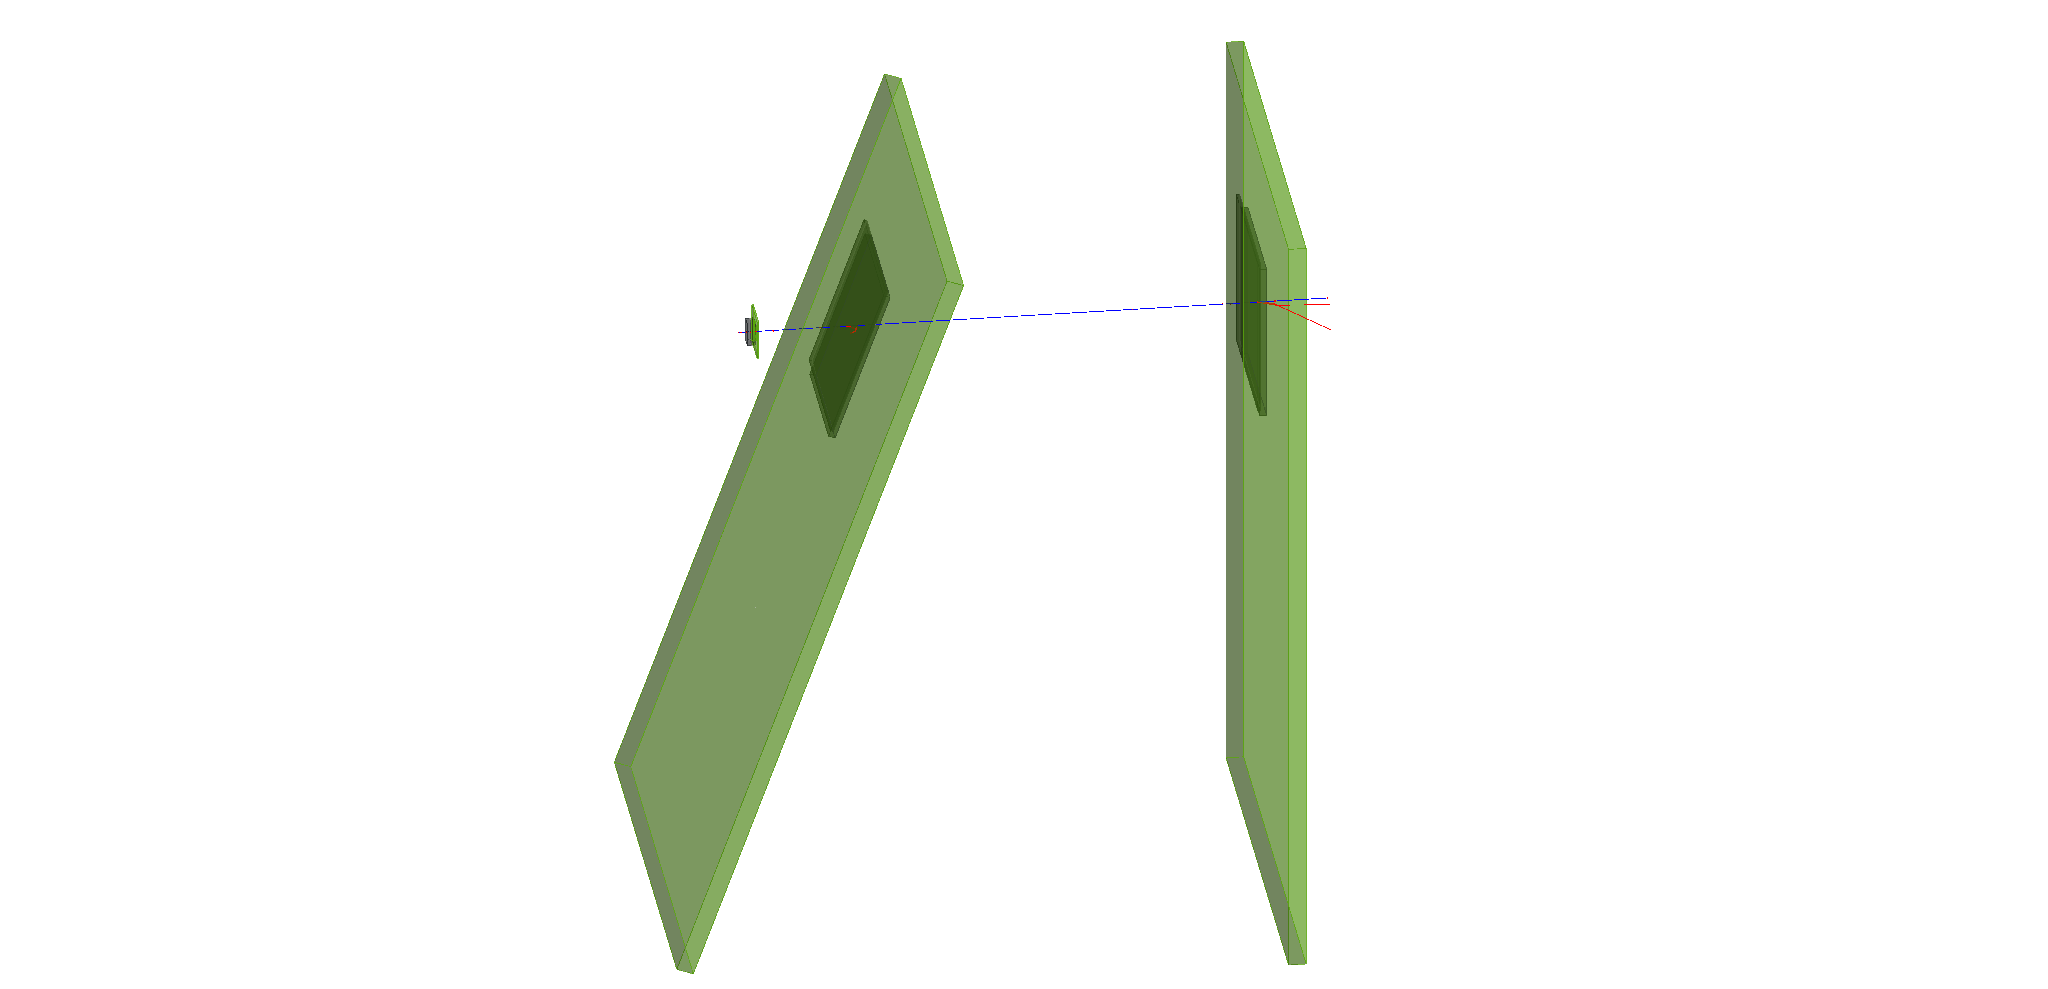
\includegraphics[width=0.6\textwidth]{telescope.png}
  \caption{Visualization of a Pion passing through the telescope setup defined in the detector configuration file. A secondary particle is produced in the material of the detector in the center.}
  \label{fig:telescope}
\end{figure}

An example configuration file describing a setup with one CLICpix2 detector and two Timepix~\cite{timepix} models is the following:
\inputminted[frame=single,framesep=3pt,breaklines=true,tabsize=2,linenos]{ini}{../../etc/manual_detector.conf}
Figure~\ref{fig:telescope} shows a visualization of the setup described in the file.
This configuration is used in the rest of this chapter for explaining concepts.

\subsubsection{Passive material configuration}
\label{sec:passive_material_config}

Descriptions of passive materials can be added to the detector setup via a set of sections, with a syntax similar to the detector configuration.
Passive geometry entries are identified by the \parameter{role} parameter set to \parameter{passive}.
Each section starts with a header describing the name used to identify the passive material; all names are required to be unique.

Every passive material has to contain all of the following parameters:
\begin{itemize}
  \item The \parameter{position} and \parameter{orientation} of the material as described for the detector, see Section \ref{sec:detector_config}.
  \item A string referring to the \parameter{type} of the passive material.
  The model should be interpreted by the module constructing the passive material, such as for example the GeometryBuilderGeant4 module.
  \item A string referring to the \parameter{material} of the passive material.
  The materials are defined in the GeometryBuilderGeant4 module and are described in the module section.
  \item A set of size parameters specific for the model that is chosen.
  All size parameters that describe the total length of something are placed such that half of this total length extends from each side of the given \parameter{position}.
  If a parameter describes the radius, this means the radius will extend from the \parameter{position} on both sides, making its total size two times the radius in the given direction.
  The size parameters for the specific models are described in Section~\ref{geometrybuildergeant4}.
\end{itemize}

In addition, an optional string referring to the \parameter{mother_volume}, which defines another passive material the volume will be placed in, can be specified.
Note: If a mother volume is chosen, the position defined in the configuration file will be relative to the center of the mother volume. An error will be given if the specified mother volume is too small for the specified size or position of this volume. Per default, the mother volume is the world frame.
Note: if the \parameter{mother_volume} is a hollow material, only the non-hollow part of the material is considered part of the material. Placing a passive volume in the hollow part requires a different \parameter{mother_volume}.

Similar to the detector configuration, the parameters \parameter{orientation_mode} (see Section~\ref{sec:models_geometry}), \parameter{alignment_precision_position} and \parameter{alignment_precision_orientation} (see Section~\ref{sec:detector_config}) can be used optionally to define the rotation order and a possible misalignment of passive materials.

An example configuration file describing a set of passive materials with different configuration options is the following:
\inputminted[frame=single,framesep=3pt,breaklines=true,tabsize=2,linenos]{ini}{../../etc/manual_passive_materials.conf}
Figure~\ref{fig:passivematerials} shows a visualization of the setup described in the file.

\begin{figure}[t]
  \centering
  \includegraphics[width=0.6\textwidth]{passive_materials.png}
  \caption{Visualization of a set of passive materials showing different configuration options.}
  \label{fig:passivematerials}
\end{figure}


\section{Framework parameters}
\label{sec:framework_parameters}
The \apsq framework provides a set of global parameters which control and alter its behavior:
\begin{itemize}
\item \parameter{detectors_file}: Location of the file describing the detector configuration (introduced in Section~\ref{sec:detector_config}).
The only \textit{required} global parameter: the framework will fail to start if it is not specified.
\item \parameter{number_of_events}: Determines the total number of events the framework should simulate.
Defaults to one (simulating a single event).
\item \parameter{skip_events}: A number of events (and therefore event seeds) to be skipped at start of the run. After skipping, the full \parameter{number_of_events} will be processed starting from the new event seed. Defaults to 0, i.e. starting with the first event seed.
\item \parameter{root_file}: Location relative to the \parameter{output_directory} where the ROOT output data of all modules will be written to. The file extension \texttt{.root} will be appended if not present.
Default value is \textit{modules.root}.
Directories within the ROOT file will be created automatically for all module instantiations.
\item \parameter{log_level}: Specifies the lowest log level which should be reported.
Possible values are \texttt{FATAL}, \texttt{STATUS}, \texttt{ERROR}, \texttt{WARNING}, \texttt{INFO}, \texttt{DEBUG}, \texttt{TRACE} and \texttt{PRNG} where all options are case-insensitive.
Defaults to the \texttt{INFO} level.
More details and information about the log levels, including how to change them for a particular module, can be found in Section~\ref{sec:logging_verbosity}.
Can be overwritten by the \texttt{-v} parameter on the command line (see Section~\ref{sec:allpix_executable}).
\item \parameter{log_format}: Determines the log message format to display.
Possible options are \texttt{SHORT}, \texttt{DEFAULT} and \texttt{LONG}, where all options are case-insensitive.
More information can be found in Section~\ref{sec:logging_verbosity}.
\item \parameter{log_file}: File where the log output should be written to in addition to printing to the standard output (usually the terminal).
Only writes to standard output if this option is not provided.
Another (additional) location to write to can be specified on the command line using the \texttt{-l} parameter (see Section~\ref{sec:allpix_executable}).
\item \parameter{output_directory}: Directory to write all output files into.
Subdirectories are created automatically for all module instantiations.
This directory will also contain the \parameter{root_file} specified via the parameter described above.
Defaults to the current working directory with the subdirectory \textit{output/} attached.
\item \parameter{purge_output_directory}: Decides whether the content of an already existing output directory is deleted before a new run starts. Defaults to \texttt{false}, i.e. files are kept but will be overwritten by new files created by the framework.
\item \parameter{deny_overwrite}: Forces the framework to abort the run and throw an exception when attempting to overwrite an existing file. Defaults to \texttt{false}, i.e. files are overwritten when requested. This setting is inherited by all modules, but can be overwritten in the configuration section of each of the modules.
\item \parameter{random_seed}: Seed for the global random seed generator used to initialize seeds for module instantiations.
The 64-bit Mersenne Twister \command{mt19937_64} from the \CPP Standard Library is used to generate seeds.
A random seed from multiple entropy sources will be generated if the parameter is not specified.
Can be used to reproduce an earlier simulation run.
\item \parameter{random_seed_core}: Optional seed used for pseudo-random number generators in the core components of the framework. If not set explicitly, the value $(\textrm{\parameter{random_seed}} + 1)$ is used.
\item \parameter{library_directories}: Additional directories to search for module libraries, before searching the default paths.
See Section~\ref{sec:module_instantiation} for details.
\item \parameter{model_paths}: Additional files or directories from which detector models should be read besides the standard search locations.
Refer to Section~\ref{sec:detector_models} for more information.
\item \parameter{performance_plots}: Enable the creation of performance plots showing the processing time required per event both for individual modules and the full module stack. Defaults to \texttt{false}.
\item \parameter{multithreading}: Enable multithreading for the framework. More information about multithreading can be found in Section~\ref{sec:multithreading}.
\item \parameter{workers}: Specify the number of workers to use in total, should be strictly larger than zero. Only used if \parameter{multithreading} is set to true. Defaults to the number of native threads available on the system if this can be determined, otherwise one thread is used.
\item \parameter{buffer_per_worker}: Specify the buffer depth available per worker for buffered modules to cache partially processed events until execution in the correct order can be guaranteed (see Section~\ref{sec:multithreading_approach}). Defaults to 512.
\end{itemize}

\section{The \textit{allpix} Executable}
\label{sec:allpix_executable}
The \parameter{allpix} executable functions as the interface between the user and the framework. It is primarily used to provide the main configuration file, but also allows to add and overwrite options from the main configuration file. This is both useful for quick testing as well as for batch processing of simulations.

The executable handles the following arguments:
\begin{itemize}
\item \texttt{-c <file>}: Specifies the configuration file to be used for the simulation, relative to the current directory.
This is the only \underline{required} argument, the simulation will fail to start if this argument is not given.
\item \texttt{-l <file>}: Specify an additional location to forward log output to, besides standard output and the location specified in the framework parameters explained in Section~\ref{sec:framework_parameters}.
\item \texttt{-v <level>}: Sets the global log verbosity level, overwriting the value specified in the configuration file described in Section~\ref{sec:framework_parameters}.
Possible values are \texttt{FATAL}, \texttt{STATUS}, \texttt{ERROR}, \texttt{WARNING}, \texttt{INFO} and \texttt{DEBUG}, where all options are case-insensitive.
The module specific logging level introduced in Section~\ref{sec:logging_verbosity} is not overwritten.
\item \texttt{-j <workers>}: Enables multithreaded event processing with the given number of worker threads. This is equivalent to passing the framework parameters \mbox{\texttt{-o multithreading=true -o workers=<workers>}} to the executable.
\item \texttt{-{}-version}: Prints the version and build time of the executable and terminates the program.
\item \texttt{-o <option>}: Passes extra framework or module options which are added and overwritten in the main configuration file.
This argument may be specified multiple times, to add multiple options.
Options are specified as key/value pairs in the same syntax as used in the configuration files (refer to Section~\ref{sec:config_file_format} for more details), but the key is extended to include a reference to a configuration section or instantiation in shorthand notation.
There are three types of keys that can be specified:
\begin{itemize}
\item Keys to set \textbf{framework parameters}. These have to be provided in exactly the same way as they would be in the main configuration file (a section does not need to be specified). An example to overwrite the standard output directory would be \texttt{allpix -c <file> -o output\_directory="run123456"}.
\item Keys for \textbf{module configurations}. These are specified by adding a dot (\texttt{.}) between the module and the actual key as it would be given in the configuration file (thus \textit{module}.\textit{key}). An example to overwrite the deposited particle to a positron would be \texttt{allpix -c <file> -o DepositionGeant4.particle\_type="e+"}.
\item Keys to specify values for a particular \textbf{module instantiation}. The identifier of the instantiation and the name of the actual key are split by a dot (\texttt{.}), in the same way as for keys for module configurations (thus \textit{identifier}.\textit{key}). The unique identifier for a module can contains one or more colons (\texttt{:}) to distinguish between various instantiations of the same module. The exact name of an identifier depends on the name of the detector and the optional input and output name. Those identifiers can be extracted from the logging section headers. An example to change the temperature of propagation for a particular instantiation for a detector named \textit{dut} could be \texttt{allpix -c <file> -o GenericPropagation:dut.temperature=273K}.
\end{itemize}
Note that only the single argument directly following the \texttt{-o} is interpreted as the option. If there is whitespace in the key/value pair this should be properly enclosed in quotation marks to ensure the argument is parsed correctly.
\item \texttt{-g <option>}: Passes extra detector options which are added and overwritten in the detector configuration file.
This argument can be specified multiple times, to add multiple options.
The options are parsed in the same way as described above for module options, but only one type of key can be specified to overwrite an option for a single detector.
These are specified by adding a dot (\texttt{.}) between the detector and the actual key as it would be given in the detector configuration file (thus \textit{detector}.\textit{key}). This method also works for customizing detector models as described in Section \ref{sec:detector_models}. An example to overwrite the sensor thickness for a particular detector named \texttt{detector1} to \texttt{50um} would be \texttt{allpix -c <file> -g detector1.sensor\_thickness=50um}.
\end{itemize}

No interaction with the framework is possible during the simulation. Signals can however be send using keyboard shortcuts to terminate the simulation, either gracefully or with force. The executable understand the following signals:
\begin{itemize}
    \item SIGINT (\texttt{CTRL+C}): Request a graceful shutdown of the simulation. This means the currently processed events are finished, while events placed on the buffer as well as all additionally requested events from the configuration file are ignored. After finishing the current events, the finalization stage is run for every module to ensure that the simulation terminates properly. This signal can be very useful when too many events are specified and the simulation takes too long to finish entirely, but the output generated so far should still be kept.
    \item SIGTERM: Same as SIGINT, request a graceful shutdown of the simulation. This signal is emitted e.g.\ by the \command{kill} command or by cluster computing schedulers to ask for a termination of the job.
    \item SIGQUIT (\texttt{CTRL+\textbackslash}): Forcefully terminates the simulation. It is not recommended to use this signal as it will normally lead to the loss of all generated data. This signal should only be used when graceful termination is for any reason not possible.
\end{itemize}


\section{Setting up the Simulation Chain}
\label{sec:setting_up_simulation_chain}

In the following, the framework parameters are used to set up a fully functional simulation.
Module parameters are shortly introduced when they are first used.
For more details about these parameters, the respective module documentation in Chapter~\ref{ch:modules} should be consulted.
A typical simulation in \apsq will contain the following components:
\begin{itemize}

\item The \textbf{geometry builder}, responsible for creating the external Geant4 geometry from the internal geometry.
In this document, \emph{internal geometry} refers to the detector parameters used by \apsq for coordinate transformations and conversions throughout the simulation, while \emph{external geometry} refers to the constructed Geant4 geometry used for charge carrier deposition (and possibly visualization).
\item The \textbf{deposition} module that simulates the particle beam creating charge carriers in the detectors using the provided physics list (containing a description of the simulated interactions) and the geometry created above.
\item A \textbf{propagation} module that propagates the charges through the sensor.
\item A \textbf{transfer} module that transfers the charges from the sensor electrodes and assigns them to a pixel of the readout electronics.
\item A \textbf{digitizer} module which converts the charges in the pixel to a detector hit, simulating the front-end electronics response.
\item An \textbf{output} module, saving the data of the simulation.
The \apsq standard file format is a ROOT TTree, which is described in detail in Section~\ref{sec:storing_output_data}.
\end{itemize}

In this example, charge carriers will be deposited in the three sensors defined in the detector configuration file in Section~\ref{sec:detector_config}.
All charge carriers deposited in the different sensors will be propagated and digitized.
Finally, monitoring histograms for the device under test (DUT) will be recorded in the framework's main ROOT file and all simulated objects, including the entry and exit positions of the simulated particles (Monte Carlo truth), will be stored in a ROOT file using the \apsq format.
An example configuration file implementing this would look like:
\inputminted[frame=single,framesep=3pt,breaklines=true,tabsize=2,linenos]{ini}{../../etc/manual.conf}

This configuration is available in the repository at \file{etc/manual.conf}.
The detector configuration file from Section~\ref{sec:detector_config} can be found at \file{etc/manual_detector.conf}.

The simulation is started by passing the path of the main configuration file to the \parameter{allpix} executable as follows:
\begin{verbatim}
$ allpix -c etc/manual.conf
\end{verbatim}
The detector histograms such as the hit map are stored in the ROOT file \file{output/modules.root} in the TDirectory \textit{DetectorHistogrammer/}.

If problems occur when exercising this example, it should be made sure that an up-to-date and properly installed version of \apsq is used (see the installation instructions in Chapter~\ref{ch:installation}).
If modules or models fail to load, more information about potential issues with the library loading can be found in the detailed framework description in Chapter~\ref{ch:framework}.

\section{Extending the Simulation Chain}
In the following, a few basic modules will be discussed which may be of use during a first simulation.

\paragraph{Visualization}
Displaying the geometry and the particle tracks helps both in checking and interpreting the results of a simulation.
Visualization is fully supported through Geant4, supporting all the options provided by Geant4~\cite{geant4vis}.
Using the Qt viewer with OpenGL driver is the recommended option as long as the installed version of Geant4 is built with Qt support enabled.

To add the visualization, the \parameter{VisualizationGeant4} section should be added at the end of the configuration file.
An example configuration with some useful parameters is given below:
\begin{minted}[frame=single,framesep=3pt,breaklines=true,tabsize=2,linenos]{ini}
[VisualizationGeant4]
# Use the Qt gui
mode = "gui"

# Set transparency of the detector models (in percent)
transparency = 0.4
# Set viewing style (alternative is 'wireframe')
view_style = "surface"

# Color trajectories by charge of the particle
trajectories_color_mode = "charge"
trajectories_color_positive = "blue"
trajectories_color_neutral = "green"
trajectories_color_negative = "red"
\end{minted}
If Qt is not available, a VRML viewer can be used as an alternative, however it is recommended to reinstall Geant4 with the Qt viewer included as it offers the best visualization capabilities.
The following steps are necessary in order to use a VRML viewer:
\begin{itemize}
\item A VRML viewer should be installed on the operating system.
Good options are FreeWRL or OpenVRML.
\item Subsequently, two environmental parameters have to be exported to the shell environment to inform Geant4 about the configuration:
\parameter{G4VRMLFILE_VIEWER} should point to the location of the viewer executable and \parameter{G4VRMLFILE_MAX_FILE_NUM} should typically be set to 1 to prevent too many files from being created.
\item Finally, the configuration section of the visualization module should be altered as follows:
\end{itemize}

\begin{minted}[frame=single,framesep=3pt,breaklines=true,tabsize=2,linenos]{ini}
[VisualizationGeant4]
# Do not start the Qt gui
mode = "none"
# Use the VRML driver
driver = "VRML2FILE"
\end{minted}

More information about all possible configuration parameters can be found in the module documentation in Chapter~\ref{ch:modules}.

\paragraph{Electric Fields}
\label{sec:module_electric_field}
By default, detectors do not have an electric field associated with them, and no bias voltage is applied.
A field can be added to each detector using the \parameter{ElectricFieldReader} module.

The section below calculates a linear electric field for every point in active sensor volume based on the depletion voltage of the sensor and the applied bias voltage.
The sensor is always depleted from the implant side; the direction of the electric field depends on the sign of the bias voltage as described in the module description in Chapter~\ref{ch:modules}.
\begin{minted}[frame=single,framesep=3pt,breaklines=true,tabsize=2,linenos]{ini}
# Add an electric field
[ElectricFieldReader]
# Set the field type to `linear`
model = "linear"
# Applied bias voltage to calculate the electric field from
bias_voltage = -50V
# Depletion voltage at which the given sensor is fully depleted
depletion_voltage = -10V
\end{minted}

\apsq also provides the possibility to utilize a full electrostatic TCAD simulation for the description of the electric field.
In order to speed up the lookup of the electric field values at different positions in the sensor, the adaptive TCAD mesh has to be interpolated and transformed into a regular grid with configurable feature size before use.
\apsq comes with a converter tool which reads TCAD DF-ISE files from the sensor simulation, interpolates the field, and writes this out in an appropriate format.
A more detailed description of the tool can be found in Section~\ref{sec:tcad_electric_field_converter}.
An example electric field (with the file name used in the example below) can be found in the \textit{etc} directory of the \apsq repository.

Electric fields can be attached to a specific detector using the standard syntax for detector binding.
A possible configuration would be:
\begin{minted}[frame=single,framesep=3pt,breaklines=true,tabsize=2,linenos]{ini}
[ElectricFieldReader]
# Bind the electric field to the detector named `dut`
name = "dut"
# Specify that the model is provided as meshed electric field map format, e.g. converted from TCAD
model = "mesh"
# Name of the file containing the electric field
file_name = "example_electric_field.init"
\end{minted}

\paragraph{Magnetic Fields}
\label{sec:module_magnetic_field}

For simulating the detector response in the presence of a magnetic field with \apsq, a constant, global magnetic field can be defined. By default, it is turned off. A field can be added to the whole setup using the unique module \parameter{MagneticFieldReader}, passing the field vector as parameter:
\begin{minted}[frame=single,framesep=3pt,breaklines=true,tabsize=2,linenos]{ini}
# Add a magnetic field
[MagneticFieldReader]
# Constant magnetic field (currently this is the default value)
model="constant"
# Magnetic field vector
magnetic_field = 0mT 3.8T 0T
\end{minted}

The global magnetic field is used by the interface to Geant4 and therefore exposes charged primary particles to the Lorentz force, and as a property of each detector present, enabling a Lorentz drift of the charge carriers in the active sensors, if supported by the used propagation modules. See Chapter \ref{ch:modules} for more information on the available propagation modules.

Currently, only constant magnetic fields can be applied.

\section{Logging and Verbosity Levels}
\label{sec:logging_verbosity}
\apsq is designed to identify mistakes and implementation errors as early as possible and to provide the user with clear indications about the problem.
The amount of feedback can be controlled using different log levels which are inclusive, i.e.\ lower levels also include messages from all higher levels.
The global log level can be set using the global parameter \parameter{log_level}.
The log level can be overridden for a specific module by adding the \parameter{log_level} parameter to the respective configuration section.
The following log levels are supported:
\begin{itemize}
\item \textbf{FATAL}: Indicates a fatal error that will lead to direct termination of the application.
Typically only emitted in the main executable after catching exceptions as they are the preferred way of fatal error handling (as discussed in Section~\ref{sec:error_reporting_exceptions}).
An example of a fatal error is an invalid configuration parameter.
\item \textbf{STATUS}: Important information about the status of the simulation.
Is only used for messages which have to be logged in every run such as the global seed for pseudo-random number generators and the current progress of the run.
\item \textbf{ERROR}: Severe error that should not occur during a normal well-configured simulation run.
Frequently leads to a fatal error and can be used to provide extra information that may help in finding the problem (for example used to indicate the reason a dynamic library cannot be loaded).
\item \textbf{WARNING}: Indicate conditions that should not occur normally and possibly lead to unexpected results.
The framework will however continue without problems after a warning.
A warning is for example issued to indicate that an output message is not used and that a module may therefore perform unnecessary work.
\item \textbf{INFO}: Information messages about the physics process of the simulation.
Contains summaries of the simulation details for every event and for the overall simulation.
Should typically produce maximum one line of output per event and module.
\item \textbf{DEBUG}: In-depth details about the progress of the simulation and all physics details of the simulation.
Produces large volumes of output per event, and should therefore only be used for  debugging the physics simulation of the modules.
\item \textbf{TRACE}: Messages to trace what the framework or a module is currently doing.
Unlike the \textbf{DEBUG} level, it does not contain any direct information about the physics of the simulation but rather indicates which part of the module or framework is currently running.
Mostly used for software debugging or determining performance bottlenecks in the simulations.
\item \textbf{PRNG}: This level enables printing of every single pseudo-random number requested from any generator used in the framework. This can be useful in order to investigate random number distribution among threads and events.
\end{itemize}

\begin{warning}
    It is not recommended to set the \parameter{log_level} higher than \textbf{WARNING} in a typical simulation as important messages may be missed.
    Setting too low logging levels should also be avoided since printing many log messages will significantly slow down the simulation.
\end{warning}

The logging system supports several formats for displaying the log messages.
The following formats are supported via the global parameter \parameter{log_format} or the individual module parameter with the same name:
\begin{itemize}
\item \textbf{SHORT}: Displays the data in a short form.
Includes only the first character of the log level followed by the configuration section header and the message.
\item \textbf{DEFAULT}: The default format.
Displays system time, log level, section header and the message itself.
\item \textbf{LONG}: Detailed logging format.
Displays all of the above but also indicates source code file and line where the log message was produced.
This can help in debugging modules.
\end{itemize}

More details about the logging system and the procedure for reporting errors in the code can be found in Sections~\ref{sec:logger} and~\ref{sec:error_reporting_exceptions}.

\section{Storing Output Data}
\label{sec:storing_output_data}
Storing the simulation output to persistent storage is of primary importance for subsequent reprocessing and analysis.
\apsq primarily uses ROOT for storing output data, given that it is a standard tool in High-Energy Physics and allows objects to be written directly to disk.
The \parameter{ROOTObjectWriter} automatically saves all objects created in a TTree~\cite{roottree}.
It stores separate trees for all object types and creates branches for every unique message name: a combination of the detector, the module and the message output name as described in Section~\ref{sec:redirect_module_input_outputs}.
For each event, values are added to the leaves of the branches containing the data of the objects.
This allows for easy histogramming of the acquired data over the total run using standard ROOT utilities.

Relations between objects within a single event are internally stored as ROOT TRefs~\cite{roottref}, allowing retrieval of related objects as long as these are loaded in memory.
An exception will be thrown when trying to access an object which is not in memory.
Refer to Section~\ref{sec:objhistory} for more information about object history.

In order to save all objects of the simulation, a \parameter{ROOTObjectWriter} module has to be added with a \parameter{file_name} parameter to specify the file location of the created ROOT file in the global output directory.
The file extension \texttt{.root} will be appended if not present.
The default file name is \texttt{data}, i.e.\ the file \textbf{data.root} is created in the output directory.
To replicate the default behaviour the following configuration can be used:
\begin{minted}[frame=single,framesep=3pt,breaklines=true,tabsize=2,linenos]{ini}
# The object writer listens to all output data
[ROOTObjectWriter]
# specify the output file (default file name is used if omitted)
file_name = "data"
\end{minted}
The generated output file can be analyzed using ROOT macros.
A simple macro for converting the results to a tree with standard branches for comparison is described in Section~\ref{sec:root_analysis_macros}.

It is also possible to read object data back in, in order to dispatch them as messages to further modules.
This feature is intended to allow splitting the execution of parts of the simulation into independent steps, which can be repeated multiple times.
The tree data can be read using a \parameter{ROOTObjectReader} module, which automatically dispatches all objects to the correct module instances.
An example configuration for using this module is:
\begin{minted}[frame=single,framesep=3pt,breaklines=true,tabsize=2,linenos]{ini}
# The object reader dispatches all objects in the tree
[ROOTObjectReader]
# path to the output data file, absolute or relative to the configuration file
file_name = "../output/data.root"
\end{minted}

The \apsq framework comes with a few more output modules which allow data storage in different formats, such as the LCIO persistency event data model~\cite{lcio}, the native RCE file format~\cite{rce}, or the Corryvreckan reconstruction framework data format.
Detailed descriptions of these modules can be found in Chapter~\ref{ch:modules}.

\cleardoublepage

% core framework
\section{The \apsq Framework}
\label{sec:framework}
The framework is split up in the following four main components that together form \apsq:
\begin{enumerate}
\item \textbf{Core}: The core contains the internal logic to initiate the modules, provide the geometry, facilitate module communication and run the event sequence. The core keeps its dependencies to a minimum (it only relies on ROOT) and remains separated from the other components as far as possibble. It is the main component discussed in this section.
\item \textbf{Modules}: A set of methods that execute a part of the simulation chain. These are build as separate libraries, loaded dynamically by the core. The available modules and their parameters are discussed in more detail in Section \ref{sec:modules}.
\item \textbf{Objects}: Objects are the data passed around between modules. They are contained into a single library and are transferred using the message framework provided by the core. Modules can listen and bind to messages they wish to receive. Messages are identified by the object type they are carrying, but they can also be named to allow redirecting data to specific modules facilitating more sophisticated simulations. Messages are meant to be read-only and a copy of the data should be made if a module wishes to change the data. More information about the messaging system and the supported objects can be found in Section \ref{sec:objects_messages}.
\item \textbf{Tools}: \apsq provides a set of header-only 'tools' that provide access to common logic shared by various modules. An example is a Eigen Runge-Kutta solver and a set of template specializations for ROOT and Geant4 configuration. More information about these can be found in Section \ref{sec:additional_tools_resources}. This set of tools is different from the set of core utilities the framework provides by itself, which are part of the core and explained in \ref{sec:logging_utilities}
\end{enumerate}
Finally \apsq provides an executable which instantiates the core, passes the configuration and runs the simulation chain.

In this chapter, first an overview of the architectural setup of the core is given and how it interacts with the total \apsq framework. Afterwards, the different subcomponents are discussed and explained in more detail. Some C++ code will be provided in the text, but readers not interested may skip the technical details.

\subsection{Architecture of the Core}
The core is constructed as a light-weight framework that provides various subsystems to the modules. It also contains the part responsible for instantiating and running the modules from the supplied configuration file. The core is structured around five subsystems of which four are centered around managers and the fifth contain a set of simple general utilities. The systems provided are:
\begin{enumerate}
\item \textbf{Configuration}: Provides a general configuration object from which data can be retrieved or stored, together with a TOML-like~\cite{tomlgit} file parser to instantiate the configurations. Also provides a general \apsq configuration manager providing access to the main configuration file and its sections. It is used by the module manager system to find the required instantiations and access the global configuration. More information is given in Section \ref{sec:config_parameters}.
\item \textbf{Module}: Contain the base class of all the \apsq modules and the manager responsible for loading and running the modules (using the configuration system). This component is discussed in more detail in Section \ref{sec:module_manager}.
\item \textbf{Geometry}: Supplies helpers for the simulation geometry. The manager contains all registered detectors. A detector has a certain position and orientation linked to an instantiation of a particular detector model. The detector model contains all parameters describing the geometry of the detector. More details about the geometry and detector models is provided in Section \ref{sec:models_geometry}.
\item \textbf{Messenger}: The messenger is responsible for sending objects from one module to another. The messenger object is passed to every module and can be used to bind to messages to listen for. Messages with objects are also dispatched through the messenger to send data to the modules listening. Please refer to Section \ref{sec:objects_messages} for more details.
\item \textbf{Utilities}: The framework provides a set of simple utilities for logging, file and directory access, random number seeding and unit conversion. An explanation how to use of these utilities can be found in Section \ref{sec:logging_utilities}. A set of C++ exceptions is also provided in the utilities, which are inherited and extended by the other components. Proper use of exceptions, together with logging informational messages and reporting errors, make the framework easier to use and debug. A few notes about the use and structure of exceptions are given in Section \ref{sec:error_reporting_exceptions}.
\end{enumerate}

\subsection{Configuration and Parameters}
\label{sec:config_parameters}
Modules and the framework are configured through configuration files. An explanation how to use the various configuration files together with several examples are provided in Section \ref{sec:configuration_files}. All configuration files follow the same format, but the way their input is interpreted differs per configuration file.

\subsubsection{File format}
\label{sec:config_file_format}
Throughout the framework a standard format is used for the configuration files, a simplified version of TOML~\cite{tomlgit}. The rules for this format are as follows:
\begin{enumerate}
\item All whitespace at the beginning or end of a line should be stripped by the parser. Empty lines should be ignored.
\item Every non-empty line should start with either \texttt{\#}, \texttt{[} or an alphanumeric character. Every other character should lead to an immediate parse error.
\item If the line starts with \texttt{\#}, it is interpreted as comment and all other content on the same line is ignored
\item If the line starts with \texttt{[}, the line indicates a section header (also known as configuration header). The line should contain an alphanumeric string indicating the header name followed by \texttt{]} to end the header (a missing \texttt{]} should raise an exception). Multiple section header with the same name are allowed. All key-value pairs following this section header are part of this section until a new section header is started. After any number of ignored whitespace characters there may be a \texttt{\#} character. If that is the case, the rest of the line is handled as specified in point~3.
\item If the line starts with an alphanumeric character, the line should indicate a key-value pair. The beginning of the line should contain an string of alphabetic characters, numbers and underscores, but note that it may not start with an underscore). This string indicates the 'key'. After a optional number of ignored whitespace, the key should be followed by an \texttt{$=$}. Any text between the \texttt{$=$} and the first \texttt{\#} character not enclosed within a pair of \texttt{"} characters is known as the non-stripped 'value'. Any character from the \texttt{\#} is handled as specified in point 3. If the line does not contain any non-enclosed \texttt{\#} character the value ends at the end of the line instead. The 'value' of the key-value pair is the non-stripped 'value' with all whitespace in front and the end stripped.
\item The value can either be accessed as a single value or an array. If the value is accessed as an array, the string is split at every whitespace or \texttt{,} character not enclosed in a pair of \texttt{"} characters. All empty entities are not considered. All other entities are treated as single values in the array.
\item All single values are stored as a string containing at least one character. The conversion to the actual type is executed when accessing the value.
\item All key-value pairs defined before the first section header are part of a zero-length empty section header
\end{enumerate}

\subsubsection{Accessing parameters}
\label{sec:accessing_parameters}
All values are accessed via the configuration object. In the following example the key is a string called \textbf{key}, the object is named \textbf{config} and the type \textbf{TYPE} is a valid C++ type that the value should represent. The values can be accessed via the following methods:
\begin{minted}[frame=single,framesep=3pt,breaklines=true,tabsize=2,linenos]{c++}
// returns true if the key exists and false otherwise
config.has("key") 
// returns the value in the given type, throws an exception if not existing
config.get<TYPE>("key") 
// returns the value in the given type or the provided default value if it does not exist
config.get<TYPE>("key", default_value) 
// returns an array of single values of the given type; throws if the key does not exist
config.getArray<TYPE>("key")
// returns an absolute (canonical if it should exist) path to a file
config.getPath("key", true /* check if path exists */)
// return an array of absolute paths
config.getPathArray("key", false /* check if paths exists */)
// returns the key as literal text including possible quotation marks
config.getText("key") 
// set the value of key to the default value if the key is not defined
config.setDefault("key", default_value) 
// set the value of the key to the defaults array if key is not defined
config.setDefaultArray<TYPE>("key", vector_of_default_values)
\end{minted}

The conversions to the type are using the \texttt{from\_string} and \texttt{to\_string} methods provided by the string utility library described in Section \ref{sec:string_utilities}. These conversions largely follows the standard C++ parsing, with one important exception. If (and only if) the value is retrieved as any C/C++ string type and the string is fully enclosed by a pair of \texttt{"} characters, they are stripped before returning the value (and strings can thus also be given without quotation marks).

\subsection{Modules and the Module Manager}
\label{sec:module_manager}
\apsq is a modular framework, the core idea is to separate functionality in various independent modules. The modules are defined in the subdirectory \textit{src/modules/} in the repository. The name of the directory is the unique name of the module. The suggested naming scheme is CamelCase, thus an example module would be \textit{GenericPropagation}. There are two different kind of modules which can be defined:
\begin{itemize}
\item \textbf{Unique}: Modules for which always a single instance runs irrespective of the number of detectors.
\item \textbf{Detector}: Modules that are specific to a single detector. They are replicated for all required detectors.
\end{itemize}
The type of module determines the kind of constructor used, the internal unique name and the supported configuration parameters. More details about the instantiation logic for the different kind of modules can be found in \ref{sec:module_instantiation}.

\subsubsection{Files of a Module}
\label{sec:module_files}
Every module directory should at the minimum contain the following documents (with \texttt{ModuleName} replaced by the name of the module):
\begin{itemize}
\item \textbf{CMakeLists.txt}: The build script to load the dependencies and define the source files
\item \textbf{README.md}: Short documentation of the module
\item \textbf{\texttt{ModuleName}.tex}: Full documentation of the module for this Users Manual
\item \textbf{\texttt{ModuleName}Module.hpp}: The header file of the module (note that another name can be used for this source file, but that is deprecated)
\item \textbf{\texttt{ModuleName}Module.cpp}: The implementation file of the module
\end{itemize}
The files are discussed in more detail below. Before the module can be used it should also be linked to the main CMakeLists.txt in \textit{src/modules/} by adding \\ ALLPIX\_BUILD\_MODULE(\texttt{ModuleName}) with the \texttt{ModuleName} being the directory of the module. 

More information about constructing new modules can be found in Section \ref{sec:building_new_module}.

\paragraph{CMakeLists.txt}
Contains the build description of the module with the following components:
\begin{enumerate}
\item On the first line either ALLPIX\_DETECTOR\_MODULE(MODULE\_NAME) or \\ ALLPIX\_UNIQUE\_MODULE(MODULE\_NAME) depending on the type of the module defined. The internal name of the module is saved to the \$\{MODULE\_NAME\} variable which should be used as argument to the other functions. Another name can be used as well, but below we exclusively use \$\{MODULE\_NAME\}
\item The next lines should contain the logic to load the dependencies of the module. Only ROOT is automatically included and linked to the module.
\item A line with ALLPIX\_MODULE\_SOURCES(\$\{MODULE\_NAME\} \texttt{sources}) where \texttt{sources} should be replaced by all the source files of this module
\item Possibly lines to include the directories and link the libraries for all the dependencies loaded in point~2.
\item A line containing ALLPIX\_MODULE\_INSTALL(\$\{MODULE\_NAME\}) to setup the required target for the module to be installed to.
\end{enumerate}

An example of a simple CMakeLists.txt of a module named \texttt{Test} which requires Geant4 is the following
\vspace{5pt}

\begin{minted}[frame=single,framesep=3pt,breaklines=true,tabsize=2,linenos]{cmake}
# Define module and save name to MODULE_NAME
# Replace by ALLPIX_DETECTOR_MODULE(MODULE_NAME) to define a detector module
ALLPIX_UNIQUE_MODULE(MODULE_NAME) 

# Load Geant4
FIND_PACKAGE(Geant4)
IF(NOT Geant4_FOUND)
    MESSAGE(FATAL_ERROR "Could not find Geant4, make sure to source the Geant4 environment\n$ source YOUR_GEANT4_DIR/bin/geant4.sh")
ENDIF()

# Add the sources for this module
ALLPIX_MODULE_SOURCES(${MODULE_NAME} 
    TestModule.cpp
)

# Add Geant4 to the include directories
TARGET_INCLUDE_DIRECTORIES(${MODULE_NAME} SYSTEM PRIVATE ${Geant4_INCLUDE_DIRS})

# Link the Geant4 libraries to the library
TARGET_LINK_LIBRARIES(${MODULE_NAME} ${Geant4_LIBRARIES})

# Provide standard install target
ALLPIX_MODULE_INSTALL(${MODULE_NAME})
\end{minted}

\paragraph{README.md}
\wip

\paragraph{\texttt{ModuleName}.tex}
\wip

\paragraph{\texttt{ModuleName}Module.hpp and \texttt{ModuleName}Module.cpp}
All modules should have both a header file and a source file. In the header file the module is defined together with all its method. Brief Doxygen documentation should be added to explain what every method does. The source file should provide the implementation of every method and also its more detailed Doxygen documentation. Not a single method should be defined in the header to keep the interface clean.

\subsubsection{Module structure}
\label{sec:module_structure}
All modules should inherit from the Module base class which can be found in \textit{src/core/module/Module.hpp}. The module base class provides two base constructors, a few convenient methods and several methods to override. Every module should provide a constructor taking a fixed set of arguments defined by the framework. This particular constructor is always called during construction by the module instantiation logic. The arguments for the constructor differs for unique and detector modules. For unique modules the constructor for a TestModule should be:
\begin{minted}[frame=single,framesep=3pt,breaklines=true,tabsize=2]{c++}
TestModule(Configuration config, Messenger* messenger, GeometryManager* geo_manager): Module(config) {}
\end{minted}
It is clear that the configuration object should be forwarded to the base module.

For unique modules the first two arguments are the same, but the last argument is a shared\_ptr to the linked detector instead. It should always forward this provided detector to the base class, besides the configuration. Thus a constructor of a detector module should be:
\begin{minted}[frame=single,framesep=3pt,breaklines=true,tabsize=2]{c++}
TestModule(Configuration config, Messenger* messenger, std::shared_ptr<Detector> detector): Module(config, detector) {}
\end{minted}

All modules receive the Configuration object holding the config parameters for that specific object, which can be accessed as explained in Section \ref{sec:accessing_parameters}. Furthermore, a pointer to the Messenger is passed which can be used to both bind variables to receive and dispatch messages as explained in \ref{sec:objects_messages}. Finally either a pointer to the GeometryManager is passed, which can be used to fetch all detectors, or a instance of the specifically linked detector. The constructor should normally be used to bind the required messages and set configuration defaults. In case of failure an exception can be thrown from the constructor. 

In addition to the constructor every module can override the following methods:
\begin{itemize}
\item \texttt{init()}: Called after loading and constructing all modules and before starting the event loop. This method can for example be used to initialize histograms.
\item \texttt{run(unsigned int event\_number)}: Called for every event in the simulation run with the event number (starting from one). An exception should be thrown for every serious error, otherwise an warning should be logged.
\item \texttt{finalize()}: Called after processing all events in the run and before destructing the module. Typically used to save the output data (like histograms). Any exceptions should be thrown from here instead of the destructor.
\end{itemize}

\subsubsection{Module instantiation}
\label{sec:module_instantiation}
The modules are dynamically loaded and instantiated by the Module Manager. Modules are constructed, initialized, executed and finalized in the linear order they are defined in the configuration file. Thus the configuration file should follow the order of the real process. For every non-special section in the main configuration file (see \ref{sec:config_parameters} for more details) a corresponding library is searched which contains the module. A module has the name \textbf{libAllPixModule\texttt{ModuleName}} reflecting the \texttt{ModuleName} of a defined module. The module search order is as follows:
\begin{enumerate}
\item The modules already loaded before from an earlier section header
\item All directories in the global configuration parameter \textit{library\_directories} in the provided order if this parameter exists
\item The internal RPATH of the executable, that should automatically point to the libraries that are build and installed together with the executable.
\item The other standard locations to search for libraries depending on the operating system, see \url{http://man7.org/linux/man-pages/man8/ld.so.8.html} for details about the procedure Linux follows.
\end{enumerate}

If the module definition is successful it is checked if the module is an unique or a detector module. The instantiation logic determines an unique name and priority, where a lower number indicates a higher priority, for every instantiation. The name and priority for the instantation are determined differently for the two types of modules:
\begin{itemize}
\item \textbf{Unique}: Combination of the name of the module and the \textbf{input} and \textbf{output} parameter (both defaulting to an empty string). The priority is always zero.
\item \textbf{Detector}: Combination of the name of the module, the \textbf{input} and \textbf{output} parameter (both defaulting to an empty string) and the name of detector this module runs on. If the name of the detector is specified directly by the \textbf{name} parameter the priority is zero. If the detector is only matched by the \textbf{type} parameter the priority is one. If the \textbf{name} and \textbf{type} are both not specified and the module is instantiated for all detectors there priority is two.
\end{itemize}
The instantiation logic only allows a single instance for every unique name. If there are multiple instantiations with the same unique name the instantiation with the highest priority is kept (thus the one with the lowest number). Otherwise if there are multiple instantiations with the same name and the same priority an exception is raised.

\subsection{Geometry and Detectors}
\label{sec:models_geometry}
Simulations are frequently run on a set of different detectors (such as as a beam telescope and a device under test). All these individual detectors together is what \apsq defines as the geometry. Every detector has a set of properties attached to it:
\begin{itemize}
\item A unique \textbf{name} to refer to the detector in the configuration.
\item The \textbf{position} in the world frame. This is the position of the geometric center of the sensitive device (sensor) given in world coordinates as X, Y and Z (note that any additional components like the chip or the PCB are ignored when determining the geometric center).
\item The \textbf{orientation} given as Euler angles using the extrinsic Z-X-Z convention relative to the world frame (also known as the 1-3-1 or the "x-convention" and the most widely used definition of Euler angles~\cite{eulerangles}). 
\item A \textbf{type} of a detector model. The model defines the geometry and parameters of the detector. Multiple detectors can share the same model (and this is in fact very common). Several ready-to-use models are shipped with the framework.
\item An optional \textbf{electric field} in the sensitive device. An electric field can be added to a detector by a special module as shown in section \ref{sec:module_electric_field}.
\end{itemize}
The detector configuration is provided in the special detector configuration which is explained in Section \ref{sec:detector_config}.

The detectors can be accessed by name through the GeometryManager. If the module is a detector-specific module its related Detector can be accessed through the \texttt{getDetector()} method (returns a null pointer for unique modules) as follows:
\begin{minted}[frame=single,framesep=3pt,breaklines=true,tabsize=2]{c++}
void run(unsigned int event_id) {
    // returns the linked detector
    std::shared_ptr<Detector> detector = this->getDetector();
}
\end{minted}

\subsubsection{Coordinate systems}
All detectors have a fixed position in the world frame which has an arbitrary origin. Every detector also has a local coordinate system attached to it. The origin of this local coordinate system does not necessarily correspond with the geometric center of the sensitive device, which is the center of orientation of the detector in the global frame. The origin of the local coordinate system is instead based on the pixel grid in the sensor. This allows for simpler calculations that are also easier to read. 

While the origin of the local coordinate system depends on the type of the model, there are fixed rules for the orientation of the coordinate system. The positive z-axis should point from the side of the sensor where collection takes place upwards (normal to the collection plane) to the other side of the sensitive device. The x-axis should point in one of the arbitrary two directions in the plane of the pixel grid. The y-axis should then be normal to both the x and the z-axis in such a way that a right-handed coordinate system is constructed. The 2D pixel grid is therefore in the XY-plane.

\subsubsection{Detector models}
\label{sec:detector_models}
Different types of detector models are already available and shipped with the framework. Every models extends from the DetectorModel base class which defines the minimum parameter of a detector model in the framework:
\begin{itemize}
\item The coordinate of the rotation center in the local frame. This is the location of the local point which is defined as position in the global frame.
\item The position of the bottom-left (minimum) of the sensor (thus the sensitive device) in the local frame. This determines the excess of the sensor and the size of the guard rings around the pixel grid. 
\item The total size of the sensor (thus the top-right corner offset from the bottom-left minimum position).
\item The number of pixels in the sensor. Every pixel is an independent block replicated over the XY plane of the sensor. The number of pixel defaults to one if it is not overridden, which means the default sensor has no replicated blocks.
\item The size of an individual pixel. The multiplication of the pixel size and the number of pixels should not exceed the sensor.
\end{itemize}

This standard detector model can be extended to provide a more detailed geometry as required by certain modules. Currently the only included advanced detector model is the PixelDetectorModel \todo{should we change this name?}, which apart from the sensor also includes guards rings, bump bonds, a readout ASIC chip, a PCB and a cover layer. 

To fetch a detector model as PixelDetectorModel, the base class should be downcasted as follows (the downcast return a null pointer if it is not a PixelDetectorModel).
\begin{minted}[frame=single,framesep=3pt,breaklines=true,tabsize=2]{c++}
// detector is a pointer to a Detector object
std::shared_ptr<PixelDetectorModel> model = std::dynamic_pointer_cast<PixelDetectorModel>(detector->getModel());
if(model != nullptr) {
    // the model of this Detector is a PixelDetectorModel
}
\end{minted}
For more details about the different types of supported models and how to add your own new model, Section \ref{sec:adding_detector_model} should be consulted.

Many detector models are shipped with the framework in the configuration format introduced in Section \ref{sec:config_file_format}. Other models can however be used in addition. To support different detector models and configuration formats the framework supports different types of model readers. These model readers search the directories in the following order:
\begin{enumerate}
\item If defined, the paths in the \textit{models\_path} parameter provided to the reader module (overridden by the global configuration \textit{models\_path}) in the given order. Files are added directly. If the path is a directory, all files in the directory are added (not recursing into subdirectories).
\item The location where the models are installed to (see the MODEL\_DIRECTORY variable in Section \ref{sec:cmake_config}). 
\item The standard data paths on the system as given by the environmental variable \$XDG\_DATA\_DIRS with the \project-directory appended. The \$XDG\_DATA\_DIRS variable defaults to \textit{/usr/local/share/} (thus effectively \textit{/usr/local/share/\project}) followed by \textit{/usr/share/} (effectively \textit{/usr/share/\project}).
\end{enumerate}
 The framework provides a DefaultModelReader module to read all the default models in the framework. Almost every simulation should include this module.

\todo{This should include more details about different model readers}

\subsection{Passing Objects using Messages}
\label{sec:objects_messages}
Communication between modules happens almost solely through messages (only some information is shared through the internally used dependencies like Geant4). Most messages are templated instantiations of the Message class carrying a vector of objects. A typedef is typically added by the object to provide an alternative name for the message directly linking to the object it is carrying. The message system has a dispatching part and a receiver part. The dispatching module can specify an optional name for the message and the receiver can also optionally specify a name to listen to. The following rules are used to dispatch the message to their receivers:
\begin{enumerate}
\item If the message type (thus usually the object type) of the receiving module does not match the type of the sending module, the message will \underline{never} be dispatched to this receiving module.
\item If the module is a detector module and the dispatched message has a detector attached, the message will \underline{never} be dispatched to this module if the detector does \underline{not} match the detector linked to the detector module.
\item If the name of the dispatched message is unspecified (or empty) the message will be dispatched to all modules (not excluded by earlier rules).
\item If the dispatched message has a specific name the message will only be dispatched to modules listening to exactly that name \underline{and} also to general listening modules that did not specify the name to receive (or set it to empty).
\end{enumerate}

An example how to dispatch a message containing an array of \textbf{Object} types, bound to a particular detector named \texttt{detector}, in the \texttt{run()} function of a certain module is provided here:
\begin{minted}[frame=single,framesep=3pt,breaklines=true,tabsize=2]{c++}
void run(unsigned int event_id) {
    std::vector<Object> data;
    // .. fill the data vector with objects ...
    
    // the last argument should be ommitted if not bound to detector
    std::shared_ptr<Message<Object>> message = std::make_shared<Message<Object>>(data, "detector");
    
    // the messenger object is a pointer to the Messenger class
    messenger->dispatchMessage(message, "" /* unnamed message */);
}
\end{minted}

\subsubsection{Methods to process messages}
The message system has multiple methods to process received messages. The first of these two are the most common methods and the third one should only rarely be used. The options are:
\begin{enumerate}
\item Bind a \textbf{single message} to a variable. This should usually be the preferred method as most modules only expect one message to arrive per event (as a module should typically send only one message containing the list of all the objects it should send). An example of how to bind a message containing an array of \textbf{Object} types in the constructor of a unique TestModule would be:
\begin{minted}[frame=single,framesep=3pt,breaklines=true,tabsize=2]{c++}
TestModule(Configuration, Messenger* messenger, GeometryManager*) {
    messenger->bindSingle(this, 
                          /* pointer to the message pointer */
                          &TestModule::message,
                          /* listen to every name */
                          "",
                          /* no message flags */
                          MsgFlags::NONE);
}
std::shared_ptr<Message<Object>> message;
\end{minted}
\item Bind a \textbf{set of messages} to an array variable. This method should be used it the module can (and expects to) receive the same message multiple times (possibly because it wants to receive the same type of message for all detectors). An example to bind multiple messages containing an array of \textbf{Object} types in the constructor of a unique TestModule would be:
\begin{minted}[frame=single,framesep=3pt,breaklines=true,tabsize=2]{c++}
TestModule(Configuration, Messenger* messenger, GeometryManager*) {
    messenger->bindMulti(this,
                          /* pointer to the message pointer */
                          &TestModule::messages,
                          /* listen to every name */
                          "",
                          /* no message flags */
                          MsgFlags::NONE);
}
std::vector<std::shared_ptr<Message<Object>>> messages;
\end{minted}
\item Listen to a particular message type and execute a \textbf{listening function} as soon as an object is received. Should be used for more advanced strategies for fetching messages. The listening module should NEVER do any heavy work in the listening function as this is supposed to take place in the run() method instead. An example of using this to listen to a message containing an array of \textbf{Object} types in a unique TestModule would be:
\begin{minted}[frame=single,framesep=3pt,breaklines=true,tabsize=2]{c++}
TestModule(Configuration, Messenger* messenger, GeometryManager*) {
    messenger->registerListener(this,
                                /* pointer to the message pointer */
                                &TestModule::listener,
                                /* listen to every name */
                                "",
                                /* no message flags */
                                MsgFlags::NONE);
}
void listener(std::shared_ptr<Message<Object>> message) {
    // do something with received message ...
}
\end{minted}
\end{enumerate}

\subsubsection{Messenger flags}
Various flags can be added to the bind function and listening functions. The flags enable a particular behaviour of the framework (if the particular type of method supports the flag).
\begin{itemize}
\item \textbf{REQUIRED}: Specify that this message is required to be received. If the particular type of message is not received before it is time to execute the run function, the run is automatically skipped by the framework. This can be used to ignore actions that would be useless without received messages, like propagating charges without any deposits.
\item \textbf{NO\_RESET}: Messages are by default automatically resetted after the run function executes to prevent older messages from previous runs to appear again. This behaviour can be disabled by setting this flag (this does not have any effect for listening functions). Setting this flag for single bound messages (without ALLOW\_OVERWRITE) would causes an exception to be raised if the message is overwritten in a later event.
\item \textbf{ALLOW\_OVERWRITE}: By default an exception is automatically raised if a single bound message is overwritten (thus set multiple times instead of once). This flag prevents this behaviour, it is only useful for single bound variables. 
\end{itemize}

\subsubsection{Object types}
All supported objects that can be transferred between modules are shipped with the framework in the Objects library. This list of objects currently consists of the following:
\begin{itemize}
\item \textbf{DepositedCharge}: Set of charges at a specific position in the sensor of a detector.
\item \textbf{PropagatedCharge}: Charge at a specific position after propagation \todo{THIS OBJECT WILL BE REMOVED?}.
\item \textbf{PixelCharge}: Set of charges at a particular pixel in the pixel grid.
\end{itemize}

\todo{this should be a separate section}

\subsection{Logging and other Utilities}
\label{sec:logging_utilities}
The \apsq framework provides a set of utilities that can be split up in two type of utilies:
\begin{itemize}
\item A few utilities to extend the functionality provided by the C++ Standard Template Library (STL). These are provided either to simplify access to the STL (like the random seed generator utility) or to provide functionality the C++14 standard lacks (like filesystem support). The referred utilities are used internally in the framework and only shortly discussed. The utilities falling in this category are the random seed generator (see Section \ref{sec:random_generator}), the filesystem functions (see Section \ref{sec:filesystem}) and the string utilies (see Section \ref{sec:string_utilities}).
\item Two utilities to improve the usability of the framework. One of these is a flexible and easy-to-use logging system, introduced below in Section \ref{sec:logger}. The other is an easy-to-use framework for units that supports converting arbitrary combinations of units to an independent number which can  be used transparently through the framework. It will be discussed in more detail in Section \ref{sec:unit_system}.
\end{itemize}

\subsubsection{Logger}
\label{sec:logger}
The logger is build to handle input/output in the same way as std::cin and std::cout do. This system is both very flexible and easy to read. It is globally configured, thus there exists only one logger and there no ocal loggers in for example a module. To send a message to the logger at a level of \textbf{LEVEL}, the following can be used:
\begin{minted}[frame=single,framesep=3pt,breaklines=true,tabsize=2,linenos]{c++}
LOG(LEVEL) << "this is an example message with data " << 1 << 2.0;
\end{minted}
Note that a newline is added at the end of every log message. Multi-line log messages can also be used: the logger will automatically align the new lines under the message itself and will leave the header space empty on the new lines.

\todo{MOVED TO GETTING STARTED}

\subsubsection{Unit system}
\label{sec:unit_system}
In physics (and therefore HEP as well) units are used a lot. Having a separate C++ type for all different kind of units would be too cumbersome for a lot of operations. Therefore the units are stored in standard C++ types in a pre-defined unit and all code in the framework uses the same unit. In various configuration files it is however very useful to give quantities in another unit. For logging it is also useful to display data in another unit.

The unit system allows adding, getting and converting units. It is a global system, thus all units should be equal through the whole framework. Examples of using the unit system are the given below:
\begin{minted}[frame=single,framesep=3pt,breaklines=true,tabsize=2,linenos]{c++}
// define the standard length unit and an auxiliary unit
Units::add("mm", 1); 
Units::add("m", 1e3); 
// define the standard time unit
Units::add("ns", 1); 
// get the units given in m/ns in the defined framework unit mm/ns
Units::get(1, "m/ns"); 
// get the framework unit of mm/ns in m/ns for logging etc
Units::convert(1, "m/ns");
\end{minted}

More details about how the unit system is used within AllPix can be found in Section \ref{sec:config_values}.

\subsubsection{Internal utilities}
\paragraph{Filesystem}
\label{sec:filesystem}
Provide functions to convert relative to absolute canonical paths, to go through all files in a directory and to create new directories. These functions should be replaced by the C++17 filesystem API\cite{cppfilesystem} as soon as the framework minimum standard is updated to C++17.

\paragraph{String utilies}
\label{sec:string_utilities}
The STL only provides string conversions for standard types using stringstream and std::to\_string. It does not allow to parse strings encapsulated in pairs of \texttt{"} characters and neither does it allow to integrate different units. Furthermore it does not provide wide flexibility to add custom conversions for other external types in both ways. The \apsq to\_string and from\_string do allow for these flexible conversions and it it extensively used in the configuration system. Conversions of numeric types with a unit attached are automatically resolved using the unit system discussed in Section \ref{sec:unit_system}. The \apsq tools system contain extensions to allow automatic conversions for ROOT and Geant4 types. The string utilities also include trim and split strings functions as they are not yet part of the STL.

\paragraph{Random seed generator}
\label{sec:random_generator}
Generating random number with a high-level of entropy is very important for running all Monte-Carlo processes in high-energy physics. Good random generators are already included in both the standard library and various external libraries. Seeding those random generators with enough entropy or seeding them with a predefined seed instead (to allow rerunning a certain simulation) should however be a framework task. This small utility library provides the required method to return a correct seed to all random generators.

\subsection{Error Reporting and Exceptions}
\label{sec:error_reporting_exceptions}
Feedback to users during the simulation is very important. The logger should be used extensively to report informational messages. Besides that reporting errors is very important. \apsq follows the principle to throw exceptions in all cases where something is wrong, it should never try to circumvent problems. Also error codes are not supposed to be used, only exceptions should be used to report fatal errors. Exceptions are also thrown for errors in the user configuration. Following this rule may lead to more frequent exceptions, but in a simulation it is typically not a problem to stop with a severe error. The asset of this method is that configuration and code is more likely to do what they are supposed to do.

The base exceptions in AllPix are defined in the utility section. The most important exception base classes are the following:
\begin{itemize}
\item \textbf{ConfigurationError}: All errors related to incorrect user configuration. Could be for example a non-existing configuration file, a missing key or an invalid parameter value.
\item \textbf{RuntimeError}: All other errrors coming up at run-time. Could be related to incorrect configuration if messages are not correctly passed or non-existing detectors are specified. Could also be raised if errors come up while loading the library or running the modules.
\item \textbf{LogicError}: Problems related to incorrectly coded modules, for example if a detector module fails to pass the detector to the constructor. These methods should never be raised for a correctly coded module and should therefore not be triggerable by users. Reporting these type of errors can help developers during their development of new modules.
\end{itemize}

\todo{add more info about error reporting style?}

\cleardoublepage

% core framework
\section{Objects}
\label{sec:objects}

\subsection{Object Types}
\label{sec:objtypes}

\apsq provides a set of objects which can be used to transfer data between modules.
These objects can be sent with the messaging system as explained in Section \ref{sec:objects_messages}.
A \texttt{typedef} is added to every object in order to provide an alternative name for the message which is directly indicating the carried object.

The list of currently supported objects comprises:
\nlparagraph{MCParticle}
The Monte-Carlo truth information about the particle passage through the sensor.
A start and end point are stored in the object: for events involving a single MCParticle passing through the sensor, the start and end points correspond to the entry and exit points.
The exact handling of non-linear particle trajectories due to multiple scattering is up to module.
The MCParticle also stores an identifier of the particle type, using the PDG particle codes~\cite{pdg}.
The MCParticle additionally stores a parent MCParticle object, if available.

\nlparagraph{DepositedCharge}
The set of charge carriers deposited by an ionizing particle crossing the active material of the sensor.
The object stores the \underline{local} position in the sensor together with the total number of deposited charges in elementary charge units.
In addition, the time (in \textit{ns} as the internal framework unit) of the deposition after the start of the event and the type of carrier (electron or hole) is stored.

\nlparagraph{PropagatedCharge}
The set of charge carriers propagated through the silicon sensor due to drift and/or diffusion processes.
The object should store the final \underline{local} position of the propagated charges.
This is either on the pixel implant (if the set of charge carriers are ready to be collected) or on any other position in the sensor if the set of charge carriers got trapped or was lost in another process.
Timing information giving the total time to arrive at the final location, from the start of the event, can also be stored.

\nlparagraph{PixelCharge}
The set of charge carriers collected at a single pixel.
The pixel indices are stored in both the $x$ and $y$ direction, starting from zero for the first pixel.
Only the total number of charges at the pixel is currently stored, the timing information of the individual charges can be retrieved from the related \parameter{PropagatedCharge} objects.

\nlparagraph{PixelHit}
The digitised pixel hits after processing in the detector's front-end electronics.
The object allows the storage of both the time and signal value.
The time can be stored in an arbitrary unit used to timestamp the hits.
The signal can hold different kinds of information depending on the type of the digitizer used.
Examples of the signal information is the 'true' information of a binary readout chip, the number of ADC counts or the ToT (time-over-threshold).

\subsection{Object History}
\label{sec:objhistory}

Objects may carry information about the objects which were used to create them.
For example, a \parameter{PropagatedCharge} could hold a link to the \parameter{DepositedCharge} object at which the propagation started.
All objects created during a single simulation event are accessible until the end of the event; more information on object persistency within the framework can be found in Section~\ref{sec:objects_persistency}. 

Object history is implemented using the ROOT TRef class~\cite{roottref}, which acts as a special reference.
On construction, every object gets a unique identifier assigned, that can be stored in other linked objects.
This identifier can be used to retrieve the history, even after the objects are written out to ROOT TTrees ~\cite{roottree}.
TRef objects are however not automatically fetched and can only be retrieved if their linked objects are available in memory, which has to be ensured explicitly.
Outside the framework this means that the relevant tree containing the linked objects should be retrieved and loaded at the same entry as the object that request the history.
Whenever the related object is not in memory (either because it is not available or not fetched) a \parameter{MissingReferenceException} will be thrown.
\cleardoublepage

% modules
\chapter{Modules}
\label{sec:modules}
This section describes all currently available \apsq modules in detail.
This includes a description of the physics implemented as well as possible configuration parameters along with their defaults.
For inquiries about certain modules or its documentation, the respective maintainers should be contacted directly.
The modules are listed in alphabetical order.

\lstset{language=Ini}
\includemodulesmd
\lstset{language=}
\cleardoublepage

% modules
\chapter{Examples}
\label{sec:examples}
This section provides brief descriptions of the example configurations currently provided in the \apsq repository.
The examples are listed in alphabetical order.

\lstset{language=Ini}
\includeexamplesmd
\lstset{language=}
\cleardoublepage

% development of new modules and detectors models
\section{Module \& Detector Development}
\subsection{Implementing a New Module}
\label{sec:building_new_module}
\subsection{Adding a New Detector Model}
\label{sec:adding_detector_model}

\cleardoublepage

\chapter{Automated Testing}
\label{ch:testing}

The build system of the framework provides a set of automated tests which are executed by the CI to ensure proper functioning of the framework and its modules.
The tests can also be manually invoked from the build directory of \apsq with
\begin{verbatim}
$ ctest
\end{verbatim}
When executed by the CI, the results on passed and failed tests are automatically gathered and prominently displayed in merge requests along with the overall CI pipeline status.
This allows a quick identification of issues without having to manually search through the log of several CI jobs.

The different subcategories of tests described below can be executed or ignored using the \command{-E} (exclude) and \command{-R} (run) switches of the \command{ctest} program:
\begin{verbatim}
$ ctest -R test_performance
\end{verbatim}

A list of all tests performed with this version of \apsq is provided in the Appendix~\ref{app:testlist}.
\section{Test Configurations}

Test configuration files consist of regular \apsq configuration files for a simulation, invoking the desired behavior to be tested.
In addition, test files can contain tags and pass conditions as described in the subsequent section.

CMake automatically searches for \apsq configuration files in the different directories and passes them to the \apsq executable~(cf.\ Section~\ref{sec:allpix_executable}).
Adding a new test is as simple as adding a new configuration file to the respective directories and specifying the pass or fail conditions based on the tags described in the following paragraphs.

Three different types of tests are distinguished:

\paragraph{Framework Functionality Tests}

The framework functionality tests validate the core framework components such as seed distribution, multithreading capabilities, configuration parsing and coordinate transformations. The configuration of the tests can be found in the \dir{etc/unittests/test_core} directory of the repository and are automatically discovered by CMake.

\paragraph{Module Functionality Tests}

These tests are meant to ensure proper functioning of an individual module given a defined input and thus protect the framework against accidental changes affecting the physics simulation.
Using a fixed seed (using the \parameter{random_seed} configuration keyword) together with a specific version of Geant4~\cite{geant4}, if necessary, allows to reproduce the same simulation event.

Typically, one single event is produced per test and the \parameter{DEBUG}-level logging output of the respective module is checked against pre-defined expectation output using regular expressions.
Once modules are altered, their respective expectation output has to be adapted after careful verification of the simulation result.

Module tests are located within the individual module source folders and are only enabled if the respective module will be built. For new modules, the directory in which the test files are located needs to be registered in the main CMake file of the module as described in Section~\ref{sec:module_files}. Module test files have to start with a two-digit number and end with the file extension \parameter{.conf}, e.g. \parameter{01-mytest.conf}, to be detected.

\paragraph{Performance Tests}

These tests run a set of simulations on a dedicated machine to catch any unexpected prolongation of the simulation time, e.g. by an accidentally introduced heavy operation in a hot loop.
Performance tests use configurations prepared such, that one particular module takes most of the load (dubbed the \emph{slowest instantiation} by \apsq), and a few of thousand events are simulated starting from a fixed seed for the pseudo-random number generator.
The \parameter{#TIMEOUT} keyword in the configuration file will ask CTest to abort the test after the given running time.

In the project CI, performance tests are limited to native runners, i.e. they are not executed on docker hosts where the hypervisor decides on the number of parallel jobs.
Only one test is performed at a time.

Despite these countermeasures, fluctuations on the CI runners occur, arising from different loads of the executing machines.
Thus, all performance CI jobs are marked with the \parameter{allow_failure} keyword which allows GitLab to continue processing the pipeline but will mark the final pipeline result as \emph{passed with warnings} indicating an issue in the pipeline.
These tests should be checked manually before merging the code under review.

The configuration of the tests can be found in the \dir{etc/unittests/test_performance} directory of the repository and are automatically discovered by CMake.

\section{Test Tags, Pass and Fail Conditions}

Test tags allow to influence the execution condition of the given test configuration, or to define a required condition for passing or failing the test.
These expressions are simply placed in the configuration file of the corresponding tests, a tag at the beginning of the line indicates which test tag the line corresponds to.
The following tags are available:

\begin{description}
  \item[Passing a test] The expression marked with the tag \parameter{#PASS} has to be found in the output in order for the test to pass. If the expression is not found, the test fails.
  \item[Failing a test] If the expression tagged with \parameter{#FAIL} is found in the output, the test fails. If the expression is not found, the test passes.
  \item[Depending on another test] The tag \parameter{#DEPENDS} can be used to indicate dependencies between tests. For example, the module test 09 described below implements such a dependency as it uses the output of module test 08-1 to read data from a previously produced \apsq data file.
  \item[Defining a timeout] For performance tests the runtime of the application is monitored, and the test fails if it exceeds the number of seconds defined using the \parameter{#TIMEOUT} tag.
  \item[Adding additional CLI options] Additional module command line options can be specified for the \parameter{allpix} executable using the \parameter{#OPTION} tag, following the format found in Section~\ref{sec:allpix_executable}. The \parameter{-o} flag will be added automatically. Multiple options can be supplied by repeating the \parameter{#OPTION} tag in the configuration file, only one option per tag is allowed. In exactly the same way options for the detectors can be set as well using the \parameter{#DETOPION} tag, where \parameter{-g} will be added automatically.
  For all other command line options to be passed to the executable, the \parameter{#CLIOPTION} can be used. Here, the complete flag and possible value needs to be passed, e.g.\ \parameter{-j9}.
  \item[Defining a test case label] Tests can be grouped and executed based on labels, e.g.\ for code coverage reports. Labels can be assigned to individual tests using the \parameter{#LABEL} tag.
\end{description}

Multiple pass or fail conditions can be separated by a semicolon or by adding multiple \parameter{#PASS} or \parameter{#FAIL} expressions.
It should however be noted that test passes or fails \emph{if any of these conditions is met}, i.e.\ the conditions are combined with a logical \parameter{OR}.
At least one pass or one fail conditions must be present in every test.

Pass and fail condition are not interpreted as regular expressions but relevant characters are automatically escaped.
This allows to directly copy corresponding lines form the log into the respective condition without manually creating a matching regular expression.
A noteworthy exception to this are line breaks.
To ease matching of multi-line expressions, the newline escape sequence \parameter{\n} of any test expression is automatically expanded to \parameter{[\r\n\t ]*} to match any new line, carriage return, tab and whitespace characters following the line break.

If no explicit fail conditions are specified, the test will fail if any \parameter{WARNING}, \parameter{ERROR} or \parameter{FATAL} appears in the output log unless it is already part of the pass condition.
For example, if a test is supposed to pass in case of an error provoked

\begin{minted}[frame=single,framesep=3pt,breaklines=true,tabsize=2,linenos]{bash}
(FATAL) [I:GeometryBuilderGeant4] Error during execution of run:
                                  Could not find a detector model of type 'missing_model'
                                  Please check your configuration and modules. Cannot continue.
\end{minted}

The full error message including the \parameter{FATAL} has to be provided as pass condition:

\begin{minted}[frame=single,framesep=3pt,breaklines=true,tabsize=2,linenos]{ini}
#PASS (FATAL) [I:GeometryBuilderGeant4] Error during execution of run:\nCould not find a detector model of type 'missing_model'
\end{minted}

If a test is expected to create multiple error or warning messages which cannot be matched with a single pass condition, the \parameter{#FAIL} parameter should be set explicitly to avoid matching the respective flags:

\begin{minted}[frame=single,framesep=3pt,breaklines=true,tabsize=2,linenos]{ini}
# This test created multiple WARNING messages, we exclude WARNING from the
# fail expression by explicitly defining it as FATAL only:
#PASS (ERROR) Multithreading disabled since the current module configuration does not support it
#FAIL FATAL
\end{minted}

\section{Directory Variables in Tests}

Sometimes it is necessary to pass directories or file names as test input.
To facilitate this, the test files can contain variables which are replaced with the respective paths before being executed.
All variable names have to be enclosed in \parameter{@} symbols to be detected and parsed correctly.
Variables can be used both in test files and the auxiliary configuration files such as detector geometry definitions.

The following variables are available:

\begin{description}
  \item[\parameter{@TEST_DIR@}:] Directory in which the current test is executed, i.e. where all output files will be placed.
  \item[\parameter{@TEST_BASE_DIR@}:] Base directory under which all tests are being executed. This can be used to reference the output files from another test. it should be noted that the respective test has to be referenced using the \parameter{#DEPENDS} keyword to ensure that it successfully ran before.
  \item[\parameter{@PROJECT_SOURCE_DIR@}:] The root directory of the project. This can for example be used to call a script provided in the \dir{etc/scripts} directory of the repository.
\end{description}

The following example demonstrates the use of these variables.
A script is called before executing the test and an input file is expected:

\begin{minted}[frame=single,framesep=3pt,breaklines=true,tabsize=2,linenos]{ini}
[Allpix]
detectors_file = "detector.conf"

[DepositionReader]
file_name = "@TEST_DIRECTORY@/deposition.root"

#BEFORE_SCRIPT python @PROJECT_SOURCE_DIR@/etc/scripts/create_deposition_file.py --type a --detector mydetector
\end{minted}

\cleardoublepage

% frequently asked question
\section{Frequently Asked Questions}
How do I run a module only for one detector?
How do I run a module only for a specific detector type?
...

\cleardoublepage

% additional tools and resources
\section{Additional Tools \& Resources}
\subsection{TCAD Electric Field Converter}
\wip
\todo{This can be added as soon it is there}

\subsection{Simple Usage Examples}
\wip
\todo{Should be filled as soon as we have some more usage examples}

\cleardoublepage

% acknowledgements to all contributors etc
\section{Acknowledgments}
We, the main contributors of \apsq (Daniel Hynds, Koen Wolters and Simon Spannagel), would like to acknowledge the contribution of the following people in particular:
\begin{itemize}
\item \textbf{Mathieu Benoit}, \textbf{John Idarraga}, \textbf{Samir Arfaoui} and all other contributors to the original AllPix, for their initial pioneering work.
\item \textbf{Neal Gauvin} for his experiments with TGeo and his help implementing a visualization module.
\item \textbf{Paul Schultze} mainly for contributing his earlier work on simulating charge propagation.
\item \textbf{Marko Petric} for his help setting up several software tools like continous integration and automatic static-code analysis.
\end{itemize}
We would also like to thank all the others that have contributed to the source code, provided input or suggested improvements. 

\cleardoublepage

\appendix
\chapter{Appendix}
\subsection{Output of Example Simulation}
\label{sec:example_output}
Possible output for the example simulation in Section \ref{sec:setting_up_simulation_chain} is given below:

\begin{lstlisting}[breaklines]
(S) Welcome to Allpix^2 v1.0beta1+110^gc065eb9
(S) Initialized PRNG with system entropy seed 11350876086373902512
(S) Loaded 8 modules
(S) Initializing 15 module instantiations
(I) [I:DepositionGeant4] Using G4 physics list "QGSP_BERT"
(I) [I:ElectricFieldReader:telescope1] Setting linear electric field from -100V bias voltage and -50V depletion voltage
(I) [I:ElectricFieldReader:dut] Setting linear electric field from -100V bias voltage and -50V depletion voltage
(I) [I:ElectricFieldReader:telescope2] Setting linear electric field from -100V bias voltage and -50V depletion voltage
(S) Initialized 15 module instantiations
(S) Running event 1 of 5
(I) [R:DepositionGeant4] Deposited 87334 charges in sensor of detector telescope1
(I) [R:DepositionGeant4] Deposited 45780 charges in sensor of detector dut
(I) [R:DepositionGeant4] Deposited 49552 charges in sensor of detector telescope2
(I) [R:GenericPropagation:dut] Propagated 22890 charges in 458 steps in average time of 3.48832ns
(I) [R:GenericPropagation:telescope2] Propagated 24776 charges in 496 steps in average time of 3.49675ns
(I) [R:SimpleTransfer:dut] Transferred 22890 charges to 4 pixels
(I) [R:SimpleTransfer:telescope2] Transferred 24776 charges to 4 pixels
(I) [R:DefaultDigitizer:dut] Digitized 2 pixel hits
(I) [R:DefaultDigitizer:telescope2] Digitized 4 pixel hits
(S) Running event 2 of 5
(I) [R:DepositionGeant4] Deposited 72234 charges in sensor of detector telescope1
(I) [R:DepositionGeant4] Deposited 56736 charges in sensor of detector dut
(I) [R:DepositionGeant4] Deposited 55882 charges in sensor of detector telescope2
(I) [R:GenericPropagation:dut] Propagated 28368 charges in 568 steps in average time of 3.49392ns
(I) [R:GenericPropagation:telescope2] Propagated 27941 charges in 559 steps in average time of 3.49617ns
(I) [R:SimpleTransfer:dut] Transferred 28368 charges to 4 pixels
(I) [R:SimpleTransfer:telescope2] Transferred 27941 charges to 4 pixels
(I) [R:DefaultDigitizer:dut] Digitized 2 pixel hits
(I) [R:DefaultDigitizer:telescope2] Digitized 4 pixel hits
(S) Running event 3 of 5
(I) [R:DepositionGeant4] Deposited 66248 charges in sensor of detector telescope1
(I) [R:DepositionGeant4] Deposited 57228 charges in sensor of detector dut
(I) [R:DepositionGeant4] Deposited 59420 charges in sensor of detector telescope2
(I) [R:GenericPropagation:dut] Propagated 28614 charges in 573 steps in average time of 3.49467ns
(I) [R:GenericPropagation:telescope2] Propagated 29710 charges in 595 steps in average time of 3.49148ns
(I) [R:SimpleTransfer:dut] Transferred 28614 charges to 3 pixels
(I) [R:SimpleTransfer:telescope2] Transferred 29710 charges to 4 pixels
(I) [R:DefaultDigitizer:dut] Digitized 2 pixel hits
(I) [R:DefaultDigitizer:telescope2] Digitized 4 pixel hits
(S) Running event 4 of 5
(I) [R:DepositionGeant4] Deposited 65206 charges in sensor of detector telescope1
(I) [R:DepositionGeant4] Deposited 70198 charges in sensor of detector dut
(I) [R:DepositionGeant4] Deposited 41846 charges in sensor of detector telescope2
(I) [R:GenericPropagation:dut] Propagated 35099 charges in 702 steps in average time of 3.49416ns
(I) [R:GenericPropagation:telescope2] Propagated 20923 charges in 419 steps in average time of 3.48176ns
(I) [R:SimpleTransfer:dut] Transferred 35099 charges to 4 pixels
(I) [R:SimpleTransfer:telescope2] Transferred 20923 charges to 4 pixels
(I) [R:DefaultDigitizer:dut] Digitized 2 pixel hits
(I) [R:DefaultDigitizer:telescope2] Digitized 4 pixel hits
(S) Running event 5 of 5
(I) [R:DepositionGeant4] Deposited 62782 charges in sensor of detector telescope1
(I) [R:DepositionGeant4] Deposited 47698 charges in sensor of detector dut
(I) [R:DepositionGeant4] Deposited 53766 charges in sensor of detector telescope2
(I) [R:GenericPropagation:dut] Propagated 23849 charges in 477 steps in average time of 3.49966ns
(I) [R:GenericPropagation:telescope2] Propagated 26883 charges in 538 steps in average time of 3.49897ns
(I) [R:SimpleTransfer:dut] Transferred 23849 charges to 3 pixels
(I) [R:SimpleTransfer:telescope2] Transferred 26883 charges to 4 pixels
(I) [R:DefaultDigitizer:dut] Digitized 2 pixel hits
(I) [R:DefaultDigitizer:telescope2] Digitized 4 pixel hits
(S) Finished run of 5 events
(I) [F:DepositionGeant4] Deposited total of 1783820 charges in 6 sensor(s) (average of 59460 per sensor for every event)
(I) [F:GenericPropagation:dut] Propagated total of 138820 charges in 2778 steps in average time of 3.4942ns
(I) [F:GenericPropagation:telescope2] Propagated total of 130233 charges in 2607 steps in average time of 3.49347ns
(I) [F:SimpleTransfer:telescope1] Transferred total of 0 charges to 0 different pixels
(I) [F:SimpleTransfer:dut] Transferred total of 138820 charges to 4 different pixels
(I) [F:SimpleTransfer:telescope2] Transferred total of 130233 charges to 4 different pixels
(I) [F:DefaultDigitizer:telescope1] Digitized 0 pixel hits in total
(I) [F:DefaultDigitizer:dut] Digitized 10 pixel hits in total
(I) [F:DefaultDigitizer:telescope2] Digitized 20 pixel hits in total
(I) [F:DetectorHistogrammer:dut] Plotted 10 hits in total, mean position is (126,125.5)
(S) [F:ROOTObjectWriter] Wrote 5498 objects to 12 branches in file:
                         /tmp/output/allpix-squared_output.root
(S) Finalization completed
(S) Executed 15 instantiations in 2 seconds, spending 58% of time in slowest instantiation DepositionGeant4
(I)  Module GeometryBuilderGeant4 took 0.0356574 seconds
(I)  Module DepositionGeant4 took 0.888584 seconds
(I)  Module ElectricFieldReader:telescope1 took 0.000102932 seconds
(I)  Module ElectricFieldReader:dut took 6.3408e-05 seconds
(I)  Module ElectricFieldReader:telescope2 took 5.5951e-05 seconds
(I)  Module DefaultDigitizer:telescope1 took 5.6189e-05 seconds
(I)  Module DefaultDigitizer:dut took 0.000543031 seconds
(I)  Module DefaultDigitizer:telescope2 took 0.000312817 seconds
(I)  Module DetectorHistogrammer:dut took 0.0237165 seconds
(I)  Module ROOTObjectWriter took 0.180625 seconds
(I)  Module SimpleTransfer:telescope1 took 6.8943e-05 seconds
(I)  Module SimpleTransfer:dut took 0.00504597 seconds
(I)  Module SimpleTransfer:telescope2 took 0.00274271 seconds
(I)  Module GenericPropagation:dut took 0.206209 seconds
(I)  Module GenericPropagation:telescope2 took 0.188115 seconds
(S) Average processing time is 306 ms/event, event generation at 3 Hz
\end{lstlisting}

% \clearpage
% \subsection{Design Development Notes}
This chapter serves as a short overview of the design goals of \apsq and the related implementation choices. Note that \apsq API is currently in a very early development stage and any implementation detail here is subject to change.

\paragraph{Goals}
\apsq is developed with a few goals in mind. These are (listed from most important to least important) the following:
\begin{enumerate}
    \item Reflects the physics
    \begin{itemize}
        \item Event based - event here refers to particle(s) passage through the setup
        \item Detectors are treated as independent objects for particles to pass through
        \item All of the information must be contained at the very end of processing an event (sequential events)
    \end{itemize}
    \item Ease of use (user-friendly)
    \begin{itemize}
        \item Simplicity for module implementation without knowing details of the framework
        \item Simple intuitive configuration and execution ("does what you expect")
    \end{itemize}
    \item Modularity
    \begin{itemize}
        \item Independent modules: write independent code without dependency on anything other but the core
        \item Allow very simple but also advanced user configurations
    \end{itemize}
    \item Flexibility
    \begin{itemize}
        \item Allow to combine different detectors, different modules
        \item Limit flexibility for the sake of simplicity and ease of use (higher on the list)
    \end{itemize}
\end{enumerate}

\paragraph{Setup}
\apsq consists of four major components listed below:
\begin{enumerate}
\item \textbf{Core}: The core contains the internal logic to initiate all modules and to run the event sequence. The core should keep its dependencies to a minimum and remain separated from the components below. More info later.
\item \textbf{Modules}: A set of methods that execute a subset of the simulation process. They are separate libraries, loaded dynamically by the core. Possible modules include one to (1) build the geometry, (2) deposit the charges in the detector, (3) propagate the charges in the detector, (4) transfer the charges to the readout chip (5) digitize the readings into a result. Furthermore there should be a set of file writer modules and (possibly) visualization modules to capture intermediate and final output. Finally there should be file input modules to simulate only a part instead of the full process.
\item \textbf{Messages}: Messages are pointers to the data passed around between the modules. Modules can listen and bind to messages they wish to receive. A message is passed around by type, but it is possible to give a message a particular name to allow modules to handle different message names (the default name is empty and dispatches the message to all modules listening to that specific type of message). Messages are meant to be read-only and a copy of the data should be made if a module developer wishes to change the data. Exact definition of the core messages is not yet provided (current ideas follow later).
\item \textbf{Tools}: \apsq will provide a simple interface to several widely used 'tools' a module wants to use. A possible example would be a runge-kutta solver.
\end{enumerate}

Finally the implementation provides a executable which integrates the core, messages and tools together with the command-line handling into a single process.

\paragraph{Core}
The core is structured around one main object (Allpix) and a set of managers. Besides this it contains a few utilities for logging, some string operations and a set of exceptions that could happen during the execution of a single event. A manager is an unique object bound to Allpix that should not be copyable. The set of managers and their uses follows hereafter.

\begin{enumerate}
\item \textbf{ConfigManager}: Loads the main configuration files and provides a set of configurations (sections) that should be converted to a set of instantiations later. The config manager should be able to provide the set of configurations in the order as they are defined in the configuration file and also allow to fetch a configuration by header. The structure of the current configuration is inspired by a simple version of \href{https://github.com/toml-lang/toml}{TOML}. The most important rules are:
\begin{itemize}
\item Every configuration start with a bracket enclosed section like \textit{[section]}.
\item Multiple sections with the same name are allowed (as long as they lead to unique instances, see below)
\item Every section contain a set of key value pairs like \textit{key = value}
\item It is up to the module developers to determine the appropriate type of the value, incorrect data should lead to an exception
\item Supported values include strings, floating-point numbers (float, double) and integers (short, int, long, long long, etc.) as well as arrays of these types
\item An array is separated by either a space or a comma
\item Extra whitespace is ignored
\item Comment lines starting with either a semicolon or a hash are ignored
\item There are a set of special key-value pairs handled by the instantiation logic instead of the module itself (see below)
\item Configurations are fixed during one run of \apsq
\item Inheriting of values from similar configurations is not yet defined... (possibly we want to inherit higher level, see part about module identifier below)
\end{itemize}
\item \textbf{ModuleManager}: Instantiates the modules from the provided configuration. Fetches the linearly defined configurations defined in the config file from the config manager. The manager dynamically loads the modules from the name specified in the configuration header. The modules should use a factory builder that creates the appropriate amount of instances for the setup. Every instantiation has a single unique identifier that may only appear once in the configuration. An identifier consist of a eventual name and type (see below) together with a potential input and output name that defaults to none, but allows to run two module with the same identifier using different inputs or output names for their messages. There are two important factories:
\begin{itemize}
\item \textbf{UniqueModuleFactory}: Creates a single instance of the module with the section header name as unique identifier. These modules should only appear once in the configuration file unless either a separate input and output name are specified.
\item \textbf{DetectorModuleFactory}: Creates a separate instance for every detector in the setup. Special configuration key/value pairs 'name' and 'type' can be provided that only build an instance for the provided detectors. A name has a higher rank than a type and should replace any comparable type instance. Creating two instances with the same identifier and the same priority is not allowed (unless their input / output name differs).
\end{itemize}
\item \textbf{GeometryManager}: Provide access to the geometry description of the detector. This needs to be provided as a simple internally defined detector description which is used by most modules. Moreover the geometry manager should provide access to a detailed detector description provider. The amount of different descriptions is not defined, but should at the minimum include a valid Geant4 description needed for the deposition of the charge carriers. The construction of the data for the geometry manager is done by the geometry builder module to allow the core to be indepedent from Geant4 etc.
\item \textbf{Messenger}: Faciliates the message passing between the modules. Messages should be the only way modules communicate with each other (besides their concurrent access of data through the managers). On instantiation modules should register for the messages they wish to receive. They can either (1) register a callback to be called on message dispatching, (2) to bind the message to variable in the class or (3) to add the message to a list of messages in the module. Messages should only be dispatched in the run() method of every module. The messenger should take care to dispatch messages to the right detector instances and match input, output names that are potentially provided.
\end{enumerate}

\paragraph{Messages}
A few ideas for messages are the following:
\begin{itemize}
\item CarrierDepositionMessage: with vector of carriers located at a certain local x,y,z position in the detector
\item CarrierCollectionMessage: with vector of carriers located at at a local x,y position on the bottom of the detector
\item CarrierTransferMessage: with vector of carriers located at a certain pixel
\item PixelHitMessage: with vector of counts of hits per pixel in a certain detector after digitizing
\end{itemize}

% \clearpage
% probably some chapter with more advanced notes

\cleardoublepage
\phantomsection
\addcontentsline{toc}{chapter}{\bibname}
% \addreferencesline
\printbibliography

\end{document}
